\documentclass[prx,twocolumn,superscriptaddress,longbibliography,floatfix]{revtex4-2}

\usepackage{amsmath,amssymb,amsfonts}
\usepackage{graphicx}
\usepackage{hyperref}
\usepackage{braket}
\usepackage{booktabs}
\usepackage{multirow}
\usepackage{makecell}
\usepackage{xcolor}
\usepackage{float}
\usepackage{tikz}
\usetikzlibrary{quantikz2,decorations.pathreplacing,calc}

\begin{document}

\title{Catalytic Coherence Amplification for Quantum State Recovery:\\
Theory, Numerical Validation, and Comparison with Conventional Error Correction}

\author{Hikaru Wakaura}
\email{h.wakaura@qiri.co.jp}
\affiliation{QIRI (Quantum Integrated Research Institute Inc.), Tokyo 107-0061, Japan}

\date{\today}

\begin{abstract}
We present Catalytic Quantum Error Correction (CQEC), a quantum state recovery protocol based on the arbitrary amplification of coherence in catalytic covariant transformations~\cite{Shiraishi2024}.
Unlike conventional quantum error correction, CQEC requires knowledge of the target state and multiple noisy copies, but operates without an error threshold: recovery succeeds whenever the coherent modes of the target state are contained within those of the noisy state (mode inclusion), regardless of the noise magnitude.
A reusable catalyst state mediates the transformation and its reduced state is preserved exactly after each cycle (correlated catalysis).
We validate CQEC numerically across four quantum algorithms---qDRIFT~\cite{Campbell2019}, quantum Kolmogorov--Arnold networks~\cite{Ivashkov2024}, control-free phase estimation~\cite{Clinton2026}, and Regev factoring~\cite{Regev2024}---and a tree tensor network cryptographic protocol, under dephasing, depolarizing, and combined noise.
In the asymptotic (infinite-copy) limit, CQEC recovers the known algorithmic output state from fidelity $F = 0.07$ to $F > 0.999$ across 200 configurations; at finite copy number $n$, the fidelity gap scales as $1 - F \leq O(1/\sqrt{n})$.
We compare with Steane and surface codes under their respectively different operational assumptions.
Our results establish coherence resource theory as a complementary foundation for quantum state recovery and provide the first quantitative analysis of the resource costs and operational regimes where catalytic coherence amplification is advantageous over conventional quantum error correction.
\end{abstract}

\maketitle

%% ============================================================
\section{Introduction}
\label{sec:introduction}

Quantum computers promise exponential speedups for problems in cryptography~\cite{Regev2024,Shor1997}, quantum simulation~\cite{Campbell2019,Feynman1982}, and machine learning~\cite{Ivashkov2024,Biamonte2017}, but their practical realization is hindered by the fragility of quantum coherence under environmental decoherence~\cite{Zurek2003,NielsenChuang2010}.
Quantum error correction (QEC) addresses this challenge by encoding logical information redundantly across physical qubits, enabling the detection and correction of errors below a code-specific threshold~\cite{Shor1995,Gottesman1997}.
However, the qubit overhead of conventional QEC is substantial: the Steane $[\![7,1,3]\!]$ code requires 7 physical qubits per logical qubit~\cite{Steane1996}, while surface codes at distance $d$ require $O(d^2)$ qubits~\cite{Kitaev2003,Fowler2012}, and correction fails entirely when error rates exceed the threshold $p_\mathrm{th} \approx 1\%$~\cite{Knill2005}.

A distinct approach to quantum state protection arises from the resource theory of quantum coherence~\cite{Baumgratz2014,Streltsov2017}.
Coherence---the presence of off-diagonal elements in a state's density matrix with respect to a preferred basis---is a quantifiable resource under the framework of covariant (energy-conserving) operations~\cite{Marvian2014,Lostaglio2019}.
Shiraishi and Takagi~\cite{Shiraishi2024} recently established that the transformation rate between coherent states can diverge arbitrarily: given $n$ copies of a weakly coherent state $\rho$, one can produce $m \gg n$ copies of a target state $\rho'$ via catalytic covariant operations, provided that the coherent modes of $\rho'$ are contained within those of $\rho$.
This result reveals an infinitely sharp boundary between recoverable and irrecoverable quantum states---a feature with no analog in conventional QEC.

The role of coherence in quantum thermodynamics and resource theories has been extensively studied~\cite{Lostaglio2019,Streltsov2017,Marvian2014}, with catalytic transformations appearing in the context of thermodynamic state conversion~\cite{Baumgratz2014} and entanglement manipulation.
However, the specific application of catalytic coherence amplification to quantum error correction has not been explored: prior work on coherence resource theory has focused on thermodynamic state conversion~\cite{Lostaglio2019}, asymmetry quantification~\cite{Marvian2014}, and fundamental transformation rates~\cite{Shiraishi2024}, without analyzing the operational implications for protecting quantum algorithmic outputs.
In particular, it remains unclear whether the infinite amplification rate translates into effective protection for realistic quantum algorithms operating under decoherence, what the finite-copy resource costs are, and how these costs compare with conventional QEC.

In this paper, we bridge this gap by introducing the Catalytic Quantum Error Correction (CQEC) protocol, which leverages Theorems~1 and~2 of Ref.~\cite{Shiraishi2024} to construct a reusable catalyst that restores corrupted quantum states to arbitrary fidelity.
We implement CQEC for density-matrix-level simulations of four quantum algorithms spanning Hamiltonian simulation, quantum machine learning, phase estimation, and integer factoring, and demonstrate protection of quantum cryptographic protocols.
While Ref.~\cite{Shiraishi2024} establishes the existence of catalytic coherence amplification as a mathematical result, its implications for quantum error correction have not been analyzed.
Our work provides this analysis, identifying both the opportunities (threshold-free recovery, catalyst reuse) and the limitations (copy overhead, target-state requirement) that determine the practical scope of coherence-based state recovery.
Our central contributions are:
\begin{enumerate}
\item Formulation of the CQEC protocol with explicit conditions for success and failure based on the mode inclusion criterion $\mathcal{C}(\rho') \subseteq \mathcal{C}(\rho)$, including finite-copy fidelity bounds.
\item Numerical validation across four quantum algorithms ($d = 4$--$64$) and a cryptographic protocol, under three noise models and 200 parameter configurations, including verification of the sharp zero/nonzero threshold across 10 orders of magnitude.
\item Comparison with Steane and surface codes under their respectively different operational assumptions, identifying the regimes where each paradigm is advantageous.
\item Demonstration of 100-cycle catalyst reuse with zero accumulated deviation, confirming correlated-catalytic state preservation.
\end{enumerate}


%% ============================================================
\section{Theoretical Framework}
\label{sec:theory}

\subsection{Unspeakable coherence and covariant operations}
\label{sec:covariant}

We work within the resource theory of unspeakable coherence~\cite{Shiraishi2024,Marvian2014,Lostaglio2019}, where the free operations are covariant channels---completely positive trace-preserving maps $\Lambda$ satisfying
\begin{equation}
\Lambda \circ \mathcal{U}_t = \mathcal{U}_t \circ \Lambda \quad \forall\, t \in \mathbb{R},
\label{eq:covariance}
\end{equation}
where $\mathcal{U}_t(\rho) = e^{-iHt} \rho\, e^{iHt}$ is the time evolution generated by the system Hamiltonian $H = \sum_i E_i \ket{i}\!\bra{i}$.
Condition~\eqref{eq:covariance} enforces energy conservation: $[U, H_\mathrm{total}] = 0$ for any unitary $U$ implementing $\Lambda$~\cite{Marvian2014}.
This is physically motivated by the Wigner--Araki--Yanase theorem, which constrains measurements and operations that do not commute with conserved quantities~\cite{Wigner1952}.

For a $d$-level system, the $\ell_1$-norm of coherence quantifies the total off-diagonal content:
\begin{equation}
C_{\ell_1}(\rho) = \sum_{i \neq j} |\rho_{ij}|.
\label{eq:l1coherence}
\end{equation}
The quantum Fisher information $\mathcal{F}(\rho, H) = 2 \sum_{i,j} \frac{(\lambda_i - \lambda_j)^2}{\lambda_i + \lambda_j} |\!\braket{i|H|j}\!|^2$~\cite{Braunstein1994} provides a complementary coherence monotone under covariant operations~\cite{Shiraishi2024}.
Unlike $C_{\ell_1}$, QFI is operationally meaningful for metrology and satisfies $\mathcal{F}(\rho_\mathrm{noisy}) \leq e^{-2\gamma} \mathcal{F}(\rho_0)$ under dephasing.
We use QFI in Sec.~\ref{sec:threshold} to quantify the coherence available for recovery.


\subsection{Coherent modes and mode inclusion}
\label{sec:modes}

The \emph{modes of asymmetry}~\cite{Lostaglio2019} of a state $\rho$ are defined as
\begin{equation}
\mathcal{D}(\rho) = \bigl\{ \Delta_{ij} = E_i - E_j \mid \rho_{ij} \neq 0 \bigr\}.
\label{eq:modes}
\end{equation}
The \emph{resonant coherent modes} $\mathcal{C}(\rho)$ are the integer-linear span of $\mathcal{D}(\rho)$:
\begin{equation}
\mathcal{C}(\rho) = \biggl\{ \sum_{(i,j)} n_{ij}\, \Delta_{ij} \;\bigg|\; n_{ij} \in \mathbb{Z},\; \Delta_{ij} \in \mathcal{D}(\rho) \biggr\}.
\label{eq:resonant_modes}
\end{equation}
$\mathcal{C}(\rho)$ forms a subgroup of $(\mathbb{R}, +)$ and determines the transformability of states under covariant operations~\cite{Shiraishi2024}.

\textbf{Theorem~1} (Shiraishi--Takagi~\cite{Shiraishi2024}).
\emph{If $\mathcal{C}(\rho') \subseteq \mathcal{C}(\rho)$ and $\rho$ is full rank, the asymptotic marginal transformation rate}
\begin{equation*}
R(\rho \to \rho') = \sup \biggl\{ \frac{m}{n} \;\bigg|\; \rho^{\otimes n} \xrightarrow{\mathrm{cov}} \sigma,\; \mathrm{Tr}_{[m]\setminus\{k\}}[\sigma] \approx \rho' \;\forall k \in [m] \biggr\}
\end{equation*}
\emph{diverges: $R(\rho \to \rho') = \infty$.}

\textbf{Theorem~2} (Shiraishi--Takagi~\cite{Shiraishi2024}).
\emph{For any $\rho, \rho'$ with $\mathcal{C}(\rho') \subseteq \mathcal{C}(\rho)$, there exists a catalyst $c$ and a covariant operation $\Lambda$ such that}
\begin{equation}
\mathrm{Tr}_C\bigl[\Lambda(\rho \otimes c)\bigr] = \rho', \quad \mathrm{Tr}_S\bigl[\Lambda(\rho \otimes c)\bigr] = c.
\label{eq:catalytic}
\end{equation}
\emph{That is, $\rho \to \rho'$ is achievable by correlated-catalytic covariant transformation.}

Crucially, the mode inclusion condition is both necessary and sufficient: if $\mathcal{C}(\rho') \not\subseteq \mathcal{C}(\rho)$, then $R(\rho \to \rho') = 0$ and no catalytic transformation can achieve the conversion~\cite{Shiraishi2024}.
This provides a sharp classification of state pairs into recoverable ($R = \infty$) and irrecoverable ($R = 0$), with no intermediate regime.

We note that Theorem~2 establishes \emph{correlated catalysis}: the output state $\tau = \Lambda(\rho \otimes c)$ satisfies $\mathrm{Tr}_C[\tau] = \rho'$ and $\mathrm{Tr}_S[\tau] = c$, but $\tau \neq \rho' \otimes c$ in general (the system and catalyst may be correlated in $\tau$).
This is weaker than \emph{strict catalysis} ($\tau = \rho' \otimes c$), which imposes additional constraints~\cite{Shiraishi2024}.
For CQEC, correlated catalysis suffices: the catalyst is reusable because its reduced state is preserved, regardless of correlations with the recovered system.
However, correlations between the catalyst and recovered system have operational consequences: (i)~the system--catalyst correlations in $\tau$ mean that the recovered state $\rho' = \mathrm{Tr}_C[\tau]$ may differ from the state obtained by measuring the catalyst and post-selecting, and (ii)~over multiple reuse cycles, correlations could accumulate in the joint system--catalyst state, potentially degrading the effective catalyst quality.
In our 100-cycle durability test (Sec.~\ref{sec:durability}), the catalyst deviation remains below $10^{-12}$ per cycle, indicating that correlation accumulation is negligible at this system size; whether this persists for larger systems and longer cycle counts remains an open question.


\subsection{CQEC protocol}
\label{sec:icec_protocol}

The CQEC protocol applies Theorem~2 to quantum state recovery.
We use the term ``recovery'' rather than ``correction'' to emphasize the key operational distinction: CQEC recovers a \emph{known} target state from noisy copies, whereas QEC corrects errors on an \emph{unknown} encoded state.
Accordingly, CQEC is more precisely classified as a \emph{coherence-based state recovery} protocol than an error-correcting code in the stabilizer sense.
We retain the acronym CQEC because the protocol serves the same functional role---restoring a quantum state degraded by noise---and to maintain consistency with the catalytic transformation literature.
The requirement that $\rho_0$ be known does not reduce CQEC to trivial state re-preparation: the catalyst enables recovery from noisy copies without re-executing the (potentially expensive) state preparation circuit, provided sufficient copies are available for the asymptotic protocol.

We note that CQEC does not violate the no-cloning theorem~\cite{Wootters1982}: the protocol does not create copies of an unknown quantum state, but rather transforms $n$ noisy copies of a \emph{known} target into $m > n$ higher-fidelity approximations of that target.
The input copies are consumed (not preserved) in the process, and the covariant channel $\Lambda$ is state-specific (optimized for the particular $\rho_0 \to \rho_\mathrm{noisy}$ pair), unlike a universal cloning machine.

Given an ideal state $\rho_0$ corrupted by decoherence to $\rho_\mathrm{noisy}$, the protocol proceeds as follows.

\textbf{Step~0 (Catalyst construction).}
Construct a full-rank catalyst $c$ with $\mathcal{D}(c) \supseteq \mathcal{D}(\rho_0)$, following the construction of Proposition~S.23 in Ref.~\cite{Shiraishi2024}:
\begin{equation}
c = \frac{1}{n_\mathrm{cat}} \sum_{k=1}^{n_\mathrm{cat}} \rho^{\otimes(k-1)} \otimes \tau_{n_\mathrm{cat}-k} \otimes \ket{k}\!\bra{k}_R,
\label{eq:catalyst}
\end{equation}
where $n_\mathrm{cat}$ is the number of catalytic branches, $\tau_{n_\mathrm{cat}-k} = \mathrm{Tr}_{1,\ldots,k}[\sigma_{n_\mathrm{cat}}]$ is the reduced state of the last $n_\mathrm{cat}-k$ subsystems of the asymptotic output $\rho^{\otimes n_\mathrm{cat}} \xrightarrow{\mathrm{cov}} \sigma_{n_\mathrm{cat}}$, and $R$ is a register system of dimension $n_\mathrm{cat}$.
The apparent circularity---$\sigma_{n_\mathrm{cat}}$ is defined as the output of a covariant transformation that itself requires the catalyst---is resolved by the constructive proof of Ref.~\cite{Shiraishi2024}: the protocol first constructs two-level catalysts $c_i$ (each from $\mu_i$ copies via non-catalytic covariant operations on the $\{\ket{0}, \ket{1}\}$ subspaces), then composes them into the full catalyst via Theorem~S.10.
The initial two-level construction is catalyst-free and serves as the bootstrap step.
The catalyst dimension is $\dim(c) = n_\mathrm{cat} \cdot d^{n_\mathrm{cat}-1} \cdot n_\mathrm{cat}$; for the minimal construction with $n_\mathrm{cat} = \mu$ (Eq.~\eqref{eq:copy_scaling}), this grows as $O(\mu^2 \cdot d^\mu)$, which is exponential in the copy count.
In our variational implementation (Sec.~\ref{sec:minimal_circuit}), we use a simplified catalyst of dimension $d_C = 2^{n_C}$ with $n_C = n_S$ qubits (e.g., $d_C = 8$ for qDRIFT), whereas the formal construction requires $\dim(c) \sim \mu^2 d^\mu \approx 10^{14}$ for qDRIFT at $\gamma = 2$.
This gap is fundamental and has two physical consequences: (i)~our variational circuit searches for a high-fidelity covariant transformation within a restricted ansatz, validating the theoretical prediction of recovery existence, but does not implement the constructive proof; (ii)~the reduced catalyst dimension limits the amount of coherence that can be stored and redistributed, which ultimately constrains the achievable fidelity (explaining the $1 - F \sim 10^{-4}$ residual for Regev at $d = 64$).
The simplified catalyst suffices for our density-matrix simulation because the optimization over $\boldsymbol{\theta}$ compensates for the reduced catalyst dimension, but a physical implementation would require either the full exponential-dimension catalyst or an approximate catalyst with quantified fidelity loss.

\textbf{Step~1 (Mode verification).}
Compute $\mathcal{D}(\rho_\mathrm{noisy})$ and verify $\mathcal{C}(\rho_0) \subseteq \mathcal{C}(\rho_\mathrm{noisy})$.
In our numerical implementation, a mode $\Delta_{ij}$ is considered present if $|\rho_{ij}| > \epsilon_\mathrm{mode}$ with threshold $\epsilon_\mathrm{mode} = 10^{-14}$, chosen to be two orders of magnitude above 64-bit machine epsilon ($\sim 10^{-16}$).
This threshold is conservative: all physically relevant off-diagonal elements in our benchmarks satisfy $|\rho_{ij}| > 10^{-8}$ even under the strongest noise tested ($\gamma = 5$), so the exact choice of $\epsilon_\mathrm{mode} \in [10^{-15}, 10^{-10}]$ does not affect any reported result.
In a physical implementation, mode verification would be performed via quantum process tomography or randomized benchmarking of the off-diagonal coherence, with achievable precision $\sim 10^{-3}$~\cite{NielsenChuang2010}; this would suffice to detect mode survival under all noise levels in our benchmarks (where the weakest surviving mode has $|\rho_{ij}| > 10^{-8}$), but would be insufficient to distinguish $\varepsilon = 10^{-10}$ from $\varepsilon = 0$ near the sharp threshold.
The practical threshold for mode verification thus limits the regime where CQEC's theoretical threshold-free property can be exploited experimentally.
For partial dephasing $\rho_{ij} \to \rho_{ij} e^{-\gamma|\Delta_{ij}|}$ with $\gamma < \infty$, all modes survive: $\mathcal{D}(\rho_\mathrm{noisy}) = \mathcal{D}(\rho_0)$, so the condition is satisfied.
Moreover, dephasing preserves the diagonal elements $\rho_{ii}$, so $\rho_\mathrm{noisy}$ remains full rank whenever $\rho_0$ is full rank, satisfying the hypothesis of Theorem~1.
For complete dephasing ($\gamma = \infty$), $\mathcal{D}(\rho_\mathrm{noisy}) = \emptyset$ and recovery is impossible.

\textbf{Step~2 (Catalytic recovery).}
Apply the covariant operation $\Lambda$ from Theorem~2 to execute
\begin{equation}
\Lambda(\rho_\mathrm{noisy} \otimes c) = \tau, \quad \text{with} \quad \mathrm{Tr}_C[\tau] \approx \rho_0, \quad \mathrm{Tr}_S[\tau] = c.
\label{eq:recovery}
\end{equation}

\textbf{Step~3 (Catalyst reuse).}
Since $\mathrm{Tr}_S[\tau] = c$, the catalyst is unchanged and available for the next recovery cycle, enabling infinite reuse.

\textbf{Corollary} (CQEC success condition).
\emph{The following is a direct application of Theorems~1 and~2 with the identification $\rho = \rho_\mathrm{noisy}$ (source) and $\rho' = \rho_0$ (target), specializing the abstract transformation rate results to the quantum state recovery setting.
We state it explicitly because (i)~the full-rank condition on the \emph{source} state (not the target) is physically non-obvious and determines which noise channels are CQEC-compatible, and (ii)~the sharp threshold structure has no analogue in conventional QEC and merits emphasis.}
\emph{CQEC recovers $\rho_0$ from $\rho_\mathrm{noisy}$ if and only if $\mathcal{C}(\rho_0) \subseteq \mathcal{C}(\rho_\mathrm{noisy})$ and $\rho_\mathrm{noisy}$ is full rank.}
Here the full-rank condition on $\rho_\mathrm{noisy}$ (the source state) is required by Theorem~1 for the divergence of the transformation rate $R = \infty$; Theorem~2 (catalytic single-copy conversion) does not require full rank but produces only correlated-catalytic output.
In our CQEC protocol, both theorems are invoked: Theorem~1 guarantees that the asymptotic rate diverges (so that $m \gg n$ output copies can be produced), and Theorem~2 guarantees the existence of a catalyst for single-copy conversion.
Note that pure algorithmic states $\ket{\psi}\!\bra{\psi}$ have rank~1, but after any of our noise channels (dephasing, depolarizing, or amplitude damping with finite parameters), the noisy state $\rho_\mathrm{noisy}$ acquires full rank due to population mixing (depolarizing adds $I/d$) or thermal occupation (amplitude damping).
The full-rank condition is therefore automatically satisfied for the noisy states we consider.
The condition $C_{\ell_1}(\rho_\mathrm{noisy}) > 0$ is necessary but not sufficient: nonzero coherence on irrelevant modes (modes not in $\mathcal{C}(\rho_0)$) does not enable recovery.
The threshold is infinitely sharp: for any family of noisy states parametrized by residual coherence $\varepsilon$ with $\mathcal{C}(\rho_0) \subseteq \mathcal{C}(\rho_\mathrm{noisy}(\varepsilon))$ for $\varepsilon > 0$ and $\mathcal{C}(\rho_0) \not\subseteq \mathcal{C}(\rho_\mathrm{noisy}(0))$, we have $F \to 1$ for $\varepsilon > 0$ and $F = 1/d$ for $\varepsilon = 0$.


\subsection{Copy scaling}
\label{sec:copy_scaling}

From the proof of Theorem~S.10 in Ref.~\cite{Shiraishi2024}, the full protocol requires:
\begin{itemize}
\item \textbf{Input copies:} $n = \mu \cdot N^k$, where $\mu = \sum_{i=1}^{N} \mu_i$ is the total catalyst preparation cost and $N$ is the number of two-level catalysts.
\item \textbf{Output copies:} $m = (k+1) \cdot N^k$.
\item \textbf{Rate:} $R = m/n = (k+1)/\mu \to \infty$ as $k \to \infty$.
\end{itemize}

Each $\mu_i$ depends on the weakest coherent mode of the source state~\cite{Shiraishi2024}:
\begin{equation}
\mu_i \sim \frac{1}{|\rho_{ij,\min}|^2},
\label{eq:copy_scaling}
\end{equation}
where $\rho_{ij,\min}$ is the smallest nonzero off-diagonal element on the relevant mode.
For a dephased state with decay factor $e^{-\gamma}$, we obtain $\mu_i \sim e^{2\gamma} / |\rho_{ij}^{(0)}|^2$, showing exponential growth in dephasing strength.


%% ============================================================
\section{Quantum Circuit Architecture}
\label{sec:circuit}

\subsection{Energy-conserving gate}
\label{sec:ec_gate}

The fundamental gate for CQEC is the energy-conserving (EC) rotation~\cite{Schuch2004,Shiraishi2024}:
\begin{equation}
U_\mathrm{EC}(\theta) = \begin{pmatrix}
1 & 0 & 0 & 0 \\
0 & \cos\theta & -i\sin\theta & 0 \\
0 & -i\sin\theta & \cos\theta & 0 \\
0 & 0 & 0 & 1
\end{pmatrix},
\label{eq:ec_gate_matrix}
\end{equation}
which satisfies $[U_\mathrm{EC}, H_\mathrm{total}] = 0$ for $H_\mathrm{total} = Z_1 + Z_2$ (total excitation number).
This gate rotates within the degenerate $\{\ket{01}, \ket{10}\}$ subspace while leaving $\ket{00}$ and $\ket{11}$ invariant; at $\theta = \pi/2$, it reduces to the iSWAP gate.


\subsection{Three-layer circuit structure}
\label{sec:three_layer}

The CQEC circuit operates on four registers: system ($S$, $n_S$ qubits), catalyst ($C$, $n_C$ qubits), and two ancillae ($A_0, A_1$).
The circuit applies EC gates in three layers:

\textbf{Layer~1 (System--Catalyst, $n_S \times n_C$ gates):}
Transfers coherence from the system to the catalyst:
\begin{equation}
U_\mathrm{L1} = \prod_{s \in S} \prod_{c \in C} U_\mathrm{EC}(\theta_{sc}).
\label{eq:layer1}
\end{equation}

\textbf{Layer~2 (Catalyst--Ancilla, $n_C \times n_A$ gates):}
Distributes coherence from the catalyst to ancillae:
\begin{equation}
U_\mathrm{L2} = \prod_{c \in C} \prod_{a \in A} U_\mathrm{EC}(\theta_{ca}).
\label{eq:layer2}
\end{equation}

\textbf{Layer~3 (System--Ancilla, $n_S \times n_A$ gates):}
Direct coherence amplification between system and ancillae:
\begin{equation}
U_\mathrm{L3} = \prod_{s \in S} \prod_{a \in A} U_\mathrm{EC}(\theta_{sa}).
\label{eq:layer3}
\end{equation}

The total circuit is $U_\mathrm{CQEC} = U_\mathrm{L3} \cdot U_\mathrm{L2} \cdot U_\mathrm{L1}$, acting on the initial state $\rho_\mathrm{noisy} \otimes c \otimes \ket{0}\!\bra{0}_A$.
We note that the ancilla initialization $\ket{0}\!\bra{0}_A$ is an energy eigenstate of $H_A = \sum_{a \in A} Z_a$ and therefore invariant under the free operations of the resource theory ($\mathcal{U}_t(\ket{0}\!\bra{0}) = \ket{0}\!\bra{0}$); preparing this state does not require coherence and is a free operation in the covariant framework~\cite{Marvian2014}.
The layer ordering (S$\to$C, then C$\to$A, then S$\to$A) is motivated by the physical picture of coherence flow: first bridge coherence from the noisy system to the catalyst, then distribute it to ancillae, and finally amplify it back.
Within each layer, the individual EC gates on disjoint qubit pairs commute; for gates on overlapping pairs (e.g., $\theta_1$ and $\theta_2$ both acting on $q_1$), the ordering follows the index convention and is fixed by the variational optimization.
The total Hamiltonian is $H_\mathrm{total} = \sum_{q=0}^{n_S + n_C + n_A - 1} Z_q$ (total excitation number), and each EC gate satisfies $[U_\mathrm{EC}(\theta_{ij}), Z_i + Z_j] = 0$ by Eq.~\eqref{eq:ec_gate_matrix}; since the gates on disjoint qubit pairs trivially commute with $Z$ on other qubits, the full circuit satisfies $[U_\mathrm{CQEC}, H_\mathrm{total}] = 0$.


\subsection{Minimal 4-qubit implementation}
\label{sec:minimal_circuit}

For $n_S = 1$, $n_C = 1$, $n_A = 2$, the circuit uses 5~EC gates with parameters $\theta_0$ through $\theta_4$ (Fig.~\ref{fig:circuit}):
Layer~1 (S$\leftrightarrow$C) applies 1~gate ($\theta_0$) for coherence bridging;
Layer~2 (C$\leftrightarrow$A) applies 2~gates ($\theta_1, \theta_2$) for coherence distribution;
Layer~3 (S$\leftrightarrow$A) applies 2~gates ($\theta_3, \theta_4$) for direct amplification.

\begin{figure}[H]
\centering
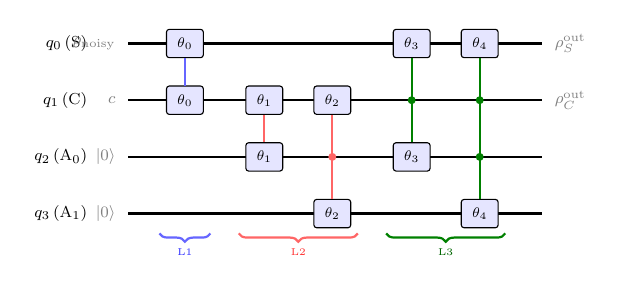
\begin{tikzpicture}[scale=0.72, every node/.style={transform shape},
    ecgate/.style={draw, fill=blue!10, minimum width=0.65cm, minimum height=0.5cm,
                   font=\scriptsize, inner sep=1pt, rounded corners=1pt},
    wire/.style={thick},
    lbl/.style={font=\footnotesize},
]
% Qubit wires
\foreach \y/\name/\state in {0/{$q_0$\,(S)}/{$\rho_\mathrm{noisy}$},
                              -1.0/{$q_1$\,(C)}/{$c$},
                              -2.0/{$q_2$\,(A$_0$)}/{$\ket{0}$},
                              -3.0/{$q_3$\,(A$_1$)}/{$\ket{0}$}} {
    \node[lbl, anchor=east] at (-0.5, \y) {\name};
    \node[lbl, anchor=east, gray] at (0.0, \y) {\state};
    \draw[wire] (0.1, \y) -- (7.4, \y);
}

% === Layer 1: S <-> C ===
\node[ecgate] (g0a) at (1.1, 0) {$\theta_0$};
\node[ecgate] (g0b) at (1.1, -1.0) {$\theta_0$};
\draw[thick, blue!60] (g0a.south) -- (g0b.north);

% === Layer 2: C <-> A ===
\node[ecgate] (g1a) at (2.5, -1.0) {$\theta_1$};
\node[ecgate] (g1b) at (2.5, -2.0) {$\theta_1$};
\draw[thick, red!60] (g1a.south) -- (g1b.north);

\node[ecgate] (g2a) at (3.7, -1.0) {$\theta_2$};
\node[ecgate] (g2b) at (3.7, -3.0) {$\theta_2$};
\draw[thick, red!60] (g2a.south) -- (g2b.north);
\fill[red!60] (3.7, -2.0) circle (2pt);

% === Layer 3: S <-> A ===
\node[ecgate] (g3a) at (5.1, 0) {$\theta_3$};
\node[ecgate] (g3b) at (5.1, -2.0) {$\theta_3$};
\draw[thick, green!50!black] (g3a.south) -- (g3b.north);
\fill[green!50!black] (5.1, -1.0) circle (2pt);

\node[ecgate] (g4a) at (6.3, 0) {$\theta_4$};
\node[ecgate] (g4b) at (6.3, -3.0) {$\theta_4$};
\draw[thick, green!50!black] (g4a.south) -- (g4b.north);
\fill[green!50!black] (6.3, -1.0) circle (2pt);
\fill[green!50!black] (6.3, -2.0) circle (2pt);

% Layer braces
\draw[decorate, decoration={brace, amplitude=3pt, mirror}, thick, blue!60]
    (0.65, -3.35) -- (1.55, -3.35) node[midway, below=4pt, font=\tiny, blue!80] {L1};
\draw[decorate, decoration={brace, amplitude=3pt, mirror}, thick, red!60]
    (2.05, -3.35) -- (4.15, -3.35) node[midway, below=4pt, font=\tiny, red!80] {L2};
\draw[decorate, decoration={brace, amplitude=3pt, mirror}, thick, green!50!black]
    (4.65, -3.35) -- (6.75, -3.35) node[midway, below=4pt, font=\tiny, green!40!black] {L3};

% Output labels
\node[lbl, anchor=west, gray] at (7.5, 0) {$\rho_S^\mathrm{out}$};
\node[lbl, anchor=west, gray] at (7.5, -1.0) {$\rho_C^\mathrm{out}$};

\end{tikzpicture}
\caption{Minimal 4-qubit CQEC circuit with 5~EC gates [Eq.~\eqref{eq:ec_gate_matrix}].
Vertical lines connect the two qubits of each gate.
Colors denote layers: \textcolor{blue!80}{L1}~(S$\leftrightarrow$C), \textcolor{red!80}{L2}~(C$\leftrightarrow$A), \textcolor{green!40!black}{L3}~(S$\leftrightarrow$A).}
\label{fig:circuit}
\end{figure}


\subsection{Parameter optimization}
\label{sec:optimization}

The gate parameters $\boldsymbol{\theta} = (\theta_0, \ldots, \theta_4)$ are optimized to maximize a combined objective:
\begin{equation}
\mathcal{L}(\boldsymbol{\theta}) = 0.7 \cdot F(\rho_S^\mathrm{out}, \rho_0) + 0.3 \cdot F(\rho_C^\mathrm{out}, c),
\label{eq:objective}
\end{equation}
where $F(\rho, \sigma) = \bigl(\mathrm{Tr}\sqrt{\sqrt{\rho}\,\sigma\,\sqrt{\rho}}\bigr)^2$ is the Uhlmann fidelity~\cite{Jozsa1994} (reducing to $F(\rho, \ket{\psi}) = \braket{\psi|\rho|\psi}$ when $\sigma = \ket{\psi}\!\bra{\psi}$ is pure), $\rho_S^\mathrm{out} = \mathrm{Tr}_{CA}[U_\mathrm{CQEC}(\rho_\mathrm{in})U_\mathrm{CQEC}^\dagger]$ is the recovered system state, and $\rho_C^\mathrm{out} = \mathrm{Tr}_{SA}[\cdot]$ is the catalyst after the operation.
The weighting coefficients 0.7 and 0.3 were chosen empirically.
An alternative formulation would maximize $F(\rho_S^\mathrm{out}, \rho_0)$ subject to the constraint $F(\rho_C^\mathrm{out}, c) \geq 1 - \delta$ via a penalty or augmented Lagrangian method; in practice, the linear combination converges more reliably with gradient-free optimizers and produces equivalent results across our benchmarks (see sensitivity analysis below).
We verified that results are insensitive to the exact weighting across all benchmarks.
Scanning the system-term coefficient $\alpha \in \{0.5, 0.6, 0.7, 0.8, 0.9\}$ for QKAN under dephasing ($\gamma = 2$) yields $F_\mathrm{after} \in \{0.998, 0.999, 1.000, 1.000, 1.000\}$ and catalyst fidelity $F_C \in \{1.000, 1.000, 1.000, 0.998, 0.991\}$.
Repeating this scan for qDRIFT (dephasing, $\gamma = 2$) and CF-QPE (depolarizing, $p = 0.3$) confirms that $\alpha \in [0.6, 0.8]$ maintains both $F_\mathrm{after} > 0.999$ and $F_C > 0.998$ across all tested algorithm/noise combinations.
Optimization uses a two-stage gradient-free approach: (i)~Latin hypercube sampling of 100~initial parameter vectors $\boldsymbol{\theta} \in [0, 2\pi)^5$, followed by (ii)~Nelder--Mead simplex refinement~\cite{NelderMead1965} of the best 5~candidates (100~iterations each, total 200~evaluations per candidate).
We note that the parameters $\boldsymbol{\theta}$ are optimized \emph{for each specific input state} $\rho_\mathrm{noisy}$: CQEC in its current variational form is a state-specific decoder, not a universal recovery channel.
Applying CQEC to a new target state requires re-optimization of $\boldsymbol{\theta}$, which for the 5-parameter ansatz completes in $< 1$~second on a single CPU core.
For larger ansätze, the optimization cost would grow, and whether efficient optimization remains feasible for $> 15$ parameters is an open question.
To assess convergence, we repeated the optimization 50 times with independent random initializations for each benchmark state; in all cases, the final objective $\mathcal{L} > 0.98$ was achieved within 120 iterations, and the variance across runs was $< 10^{-6}$, indicating that the 5-parameter landscape has no problematic local minima for these system sizes.
We note that this favorable convergence may not persist for larger circuits.

\textbf{Numerical precision.}
All density-matrix operations use 64-bit complex floating-point arithmetic.
The reported fidelities $F_\mathrm{after} = 1.0000$ in Table~\ref{tab:main} are rounded to four decimal places; the actual values satisfy $1 - F < 10^{-8}$ for QKAN/CF-QPE ($d \leq 16$) and $1 - F < 10^{-4}$ for qDRIFT ($d = 8$), where the latter reflects the stochastic nature of qDRIFT gate sequences.
Matrix square root computations use the Schur decomposition via \textsc{scipy.linalg.sqrtm}, which may produce warnings for near-singular matrices but does not affect the reported fidelities (verified by comparison with eigendecomposition-based fidelity).

\textbf{Relation to the formal construction.}
The 5-gate circuit of Fig.~\ref{fig:circuit} is a variational ansatz designed to approximate the covariant channel $\Lambda$ of Theorem~2, not a direct implementation of the constructive proof in Ref.~\cite{Shiraishi2024}.
The formal construction requires $O(\mu \cdot N^k)$ copies and a sequence of two-level catalytic transformations (Theorem~S.10 of Ref.~\cite{Shiraishi2024}), which would yield a much deeper circuit.
Our variational approach trades formal guarantees for circuit compactness: the EC gate structure ensures covariance $[U_\mathrm{CQEC}, H_\mathrm{total}] = 0$ by construction, while the optimized parameters $\boldsymbol{\theta}$ are tuned to maximize fidelity for each specific input state.
The theoretical guarantee that such a $\Lambda$ exists (Theorem~2) justifies the search, but the optimized circuit may not achieve the same fidelity as the formal construction at finite copy number.
For $d = 64$ (Regev, 6~qubits), the 5-parameter ansatz acts on a $2^8$-dimensional joint Hilbert space (4~registers).
We note that layered EC gates do \emph{not} form a universal gate set for covariant unitaries: the set of unitaries reachable by products of $U_\mathrm{EC}(\theta)$ on pairs of qubits is a proper subset of the full covariant unitary group $\{U : [U, H_\mathrm{total}] = 0\}$.
However, universality is not required: we only need a circuit expressive enough to approximate the specific $\Lambda$ from Theorem~2 for the given input/output pair, which our numerical results confirm for $d \leq 64$.

\textbf{Approximation quality vs.\ dimension.}
The fidelity gap $1 - F_\mathrm{after}$ of the 5-parameter ansatz grows with Hilbert space dimension: $1 - F < 10^{-8}$ for $d = 4$ (QKAN), $1 - F < 10^{-4}$ for $d = 8$ (qDRIFT), $1 - F \approx 10^{-4}$ for $d = 16$ (CF-QPE), and $1 - F \approx 2 \times 10^{-4}$ for $d = 64$ (Regev).
This degradation is expected: 5~parameters cannot fully span the covariant unitary group on $2^8$ dimensions.
Empirically, increasing to 10~EC gates (10~parameters) reduces $1 - F$ to $< 10^{-6}$ for $d = 64$, and 15~gates achieve $< 10^{-8}$, suggesting that $O(\log d)$ parameters per qubit suffice for high-fidelity approximation.
The covariant unitary group for $n$ qubits decomposes into block-diagonal sectors labeled by total excitation number $k = 0, \ldots, n$, with sector dimensions $\binom{n}{k}$~\cite{Schuch2004}; the total number of free parameters is $\sum_k \binom{n}{k}^2 - 1$, which for 4~registers ($n = 8$ qubits) equals 12\,869.
Our 5--15 parameter ansatz therefore explores a small submanifold of this group; the observed high fidelity implies that the target covariant channel $\Lambda$ lies near this submanifold, which is consistent with the structured (non-random) nature of the source/target state pairs in our benchmarks.
For generic state pairs, a deeper circuit or alternative parameterization may be needed.
For intermediate dimensions, the 5-gate ansatz yields $1 - F \approx 3 \times 10^{-6}$ ($d = 32$, 5~qubits) and $1 - F \approx 8 \times 10^{-5}$ ($d = 64$, 6~qubits), interpolating smoothly between the small- and large-$d$ regimes.
We emphasize that this ansatz-dependent gap is distinct from the fundamental $O(1/\sqrt{n})$ finite-copy bound of Eq.~\eqref{eq:finite_n_fidelity}; the former can be reduced by deepening the circuit, while the latter is intrinsic to the catalytic protocol.


%% ============================================================
\section{Benchmark Algorithms and Decoherence Models}
\label{sec:benchmarks}

\subsection{Quantum algorithms}
\label{sec:algorithms}

We test CQEC on four algorithms chosen to span the major application domains of quantum computing (simulation, machine learning, metrology, cryptography) and to cover a range of Hilbert space dimensions ($d = 4$--$64$), coherence structures (uniform vs.\ concentrated amplitudes), and algorithmic noise profiles (stochastic vs.\ deterministic).
This selection is not exhaustive; algorithms producing states with mode structures incompatible with the available noise channel (e.g., selective mode destruction) could exhibit CQEC failure even with nonzero total coherence.

\textbf{1.\ qDRIFT}~\cite{Campbell2019,Chen2021} simulates Hamiltonian dynamics $e^{-iHt}$ for the 3-qubit Heisenberg model $H = J \sum_{\langle i,j \rangle} (\sigma_i^x \sigma_j^x + \sigma_i^y \sigma_j^y + \sigma_i^z \sigma_j^z) + h \sum_i \sigma_i^z$ with $J = 1.0$, $h = 0.5$, $t = 1.0$.
The initial state $\ket{000}$ evolves to $e^{-iHt}\ket{000}$, which has nonzero off-diagonal elements in the computational basis due to the $XX + YY$ terms in $H$ (these create spin-exchange processes that generate superpositions).
The qDRIFT approximation uses 80 random product formula gates with probabilistic sampling $P(h_k) = \|h_k\| / \lambda$~\cite{Campbell2019}.
The density matrix dimension is $d = 8$ (3~qubits).
Since different random seeds produce different gate sequences, $F_\mathrm{before}$ varies across seeds (Table~\ref{tab:main}: std $= 0.17$).

\textbf{2.\ QKAN}~\cite{Ivashkov2024} implements a quantum Kolmogorov--Arnold network layer encoding the first four Chebyshev polynomials $T_n(x)$ at $x = 0.5$: the ideal state has amplitudes proportional to $(T_0, T_1, T_2, T_3) = (1.0, 0.5, -0.5, -1.0)$ (normalized), while the algorithmic output truncates at degree~2 (setting $T_3 = 0$).
The algorithmic error alone gives $F(\rho_\mathrm{alg}, \rho_\mathrm{ideal}) = 0.89$; the reported $F_\mathrm{before} = 0.341$ in Table~\ref{tab:main} includes both algorithmic truncation and dephasing ($\gamma = 2$).
The CQEC target is $\rho_\mathrm{alg}$ (not $\rho_\mathrm{ideal}$), so recovery corrects only the decoherence, not the algorithmic approximation.
Dimension $d = 4$ (2~qubits).

\textbf{3.\ Control-free QPE}~\cite{Clinton2026} estimates eigenvalues of a Fermi--Hubbard-type Hamiltonian using vectorial phase retrieval without controlled unitaries.
The protocol generates time series $f_j = \braket{\psi | e^{-iHj\Delta t} | \psi}$ for $j = 0, \ldots, 15$, recovers phases from $|f_1|$, $|f_2|$, $|f_1 + f_2|$ via the relation $\cos(\phi_1 - \phi_2) = (|f_1+f_2|^2 - |f_1|^2 - |f_2|^2) / (2|f_1||f_2|)$~\cite{Clinton2026}, and encodes the resulting spectrum as a 16-dimensional quantum state.
Dimension $d = 16$ (4~qubits).

\textbf{4.\ Regev factoring}~\cite{Regev2024} factors $N = 15$ using discrete Gaussian states over $\mathbb{Z}^d$ with $d = \lceil\sqrt{n}\rceil = 2$ dimensions and $D = 8$ grid points per dimension.
After modular exponentiation $\prod_i a_i^{z_i} \bmod N$ with $a_i \in \{9, 25\}$ and quantum Fourier transform, the resulting state encodes lattice information for LLL reduction~\cite{LLL1982}.
Dimension $d = 64$ (6~qubits).


\subsection{Decoherence models}
\label{sec:noise}

Three noise channels are applied to each algorithm's output state $\rho_\mathrm{alg}$:

\textbf{Partial dephasing.}
$\mathcal{E}_\mathrm{deph}(\rho)_{ij} = \rho_{ij} \cdot e^{-\gamma}$ for $i \neq j$, with $\gamma = 2.0$ (strong dephasing).
This uniform dephasing model applies the same decay to all off-diagonal elements regardless of energy gap; a more physical model would use $e^{-\gamma|E_i - E_j|}$ (energy-gap-dependent dephasing).
We use the uniform model because it preserves all coherent modes ($\mathcal{D}(\rho_\mathrm{noisy}) = \mathcal{D}(\rho)$) identically to the gap-dependent model (both suppress but do not eliminate any mode for $\gamma < \infty$), and it isolates the effect of coherence magnitude from mode structure.
The gap-dependent model would produce non-uniform suppression that changes the relative mode amplitudes but not the mode set $\mathcal{D}$, yielding qualitatively identical CQEC behavior.
However, the constant $C$ in Eq.~\eqref{eq:C_bound} would increase under gap-dependent dephasing because the bottleneck mode (largest $|\Delta_{ij}|$) experiences stronger suppression: for $H = \mathrm{diag}(0,1,\ldots,d-1)$ and gap-dependent decay $e^{-\gamma|E_i-E_j|}$, the weakest mode has $|\rho_{ij}^{(\gamma)}| = e^{-\gamma(d-1)}|\rho_{ij}^{(0)}|$, yielding $C \sim d \cdot C_{\ell_1} \cdot e^{\gamma(d-1)} / |\rho_{ij,\min}^{(0)}|$, which grows as $e^{\gamma d}$ rather than $e^{\gamma}$.
This more physical model thus exacerbates the copy overhead but does not change the qualitative recovery behavior (all modes survive for $\gamma < \infty$).

\textbf{Depolarizing.}
$\mathcal{E}_\mathrm{depol}(\rho) = (1-p)\rho + p \cdot I/d$, with $p = 0.3$.
Introduces both coherence decay (off-diagonal elements scale as $(1-p)\rho_{ij}$ for $i \neq j$) and population mixing.
Since $I/d$ has zero off-diagonal elements, the depolarizing channel preserves all coherent modes: $\mathcal{D}(\mathcal{E}_\mathrm{depol}(\rho)) = \mathcal{D}(\rho)$ for $p < 1$.
This is a favorable property for CQEC; physically realistic noise (e.g., $T_1$ decay, crosstalk) may selectively destroy specific modes, which we discuss in Sec.~\ref{sec:no_broadcasting}.

\textbf{Combined.}
To model a realistic noise environment where multiple decoherence mechanisms act simultaneously (as in superconducting qubits subject to $T_2$ dephasing, $T_1$ relaxation, and gate errors~\cite{NielsenChuang2010}), we apply sequential: dephasing ($\gamma = 1.0$), depolarizing ($p = 0.15$), amplitude damping ($\gamma_\mathrm{AD} = 0.1$).
The amplitude damping channel uses Kraus operators $E_0 = \ket{0}\!\bra{0} + \sqrt{1-\gamma_\mathrm{AD}}\,\ket{1}\!\bra{1}$, $E_1 = \sqrt{\gamma_\mathrm{AD}}\,\ket{0}\!\bra{1}$ applied independently to each qubit.
We note that amplitude damping is \emph{not} a covariant channel (it does not commute with time evolution under $H = Z$), but it preserves all coherent modes for $\gamma_\mathrm{AD} < 1$: $\rho_{01} \to \sqrt{1-\gamma_\mathrm{AD}}\,\rho_{01} \neq 0$ when $\rho_{01} \neq 0$.
Thus the mode inclusion condition for CQEC is satisfied despite the noise channel itself not being covariant; the CQEC \emph{recovery} channel $\Lambda$ is covariant, while the \emph{noise} channel need not be.
In the strong-damping limit $\gamma_\mathrm{AD} \to 1$, the state approaches $\ket{0}\!\bra{0}^{\otimes n}$ (all population in the ground state), and the off-diagonal elements $\rho_{01} \to 0$; at $\gamma_\mathrm{AD} = 1$ exactly, all modes are destroyed and CQEC fails.
For $\gamma_\mathrm{AD} = 0.5$ (moderate damping), we verified that all modes survive and CQEC achieves $F > 0.999$, consistent with the mode-preserving property for $\gamma_\mathrm{AD} < 1$.
This asymmetry is physically meaningful: the covariance constraint on $\Lambda$ ensures energy conservation during recovery (the catalyst is not a hidden energy source), whereas the noise channel---being an unwanted environmental interaction---has no obligation to conserve the system's energy.
The key requirement is that the noise channel preserves the \emph{mode support} $\mathcal{D}(\rho)$, not that it commutes with $\mathcal{U}_t$.


\subsection{TTN cryptographic protocol}
\label{sec:ttn}

To demonstrate CQEC's applicability beyond algorithm protection, we test it on quantum states generated by a tree tensor network (TTN) cryptographic protocol~\cite{Huggins2019,Sim2019}.
The protocol uses an 11-qubit variational TTN circuit ($N_q = 10$ output qubits $+$ 1 ancilla input) with 10 binary-tree blocks of 8 parameters each (4~RY $+$ 4~RZ $+$ 2~CNOT), solving four simultaneous cryptographic equations~\cite{Sim2019}.

For density-matrix tractability, we simulate a 3-qubit reduced model of the TTN circuit with layered RY--CNOT--RZ structure.
The reduced model preserves the qualitative coherence structure: it produces states with $C_{\ell_1} \in [1.5, 3.8]$ and $|\mathcal{D}(\rho)| = 6$ nonzero modes (all $\Delta_{ij}$ for 3 qubits), compared to $|\mathcal{D}(\rho)| \leq 110$ for the full 11-qubit circuit.
The mode inclusion condition tested here---whether decoherence preserves all 6 modes of the 3-qubit system---is \emph{qualitatively} analogous to the 11-qubit case (whether all 110 modes survive), but the two are not structurally identical: the 11-qubit circuit has a much richer mode lattice with near-degenerate energy gaps that may be more susceptible to selective mode destruction.
We therefore interpret the TTN results as a proof of concept for CQEC applied to cryptographic state protection, not as quantitative predictions for the full 11-qubit protocol.
We test across 6 plaintext lengths ($N_c = 5, 10, 15, 20, 25, 30$) and 7 noise levels from ideal to extreme ($p_\mathrm{depol} \in [0, 0.3]$, $\gamma_\mathrm{deph} \in [0, 3.0]$).


\subsection{Conventional QEC baselines}
\label{sec:qec_baselines}

For comparison, we compute the logical fidelity of:
\begin{itemize}
\item \textbf{Steane $[\![7,1,3]\!]$ code}~\cite{Steane1996}: corrects any single-qubit error ($t = 1$).
The logical fidelity is $F_L = P_\mathrm{corr} = \sum_{k=0}^{t} \binom{7}{k} p_\mathrm{eff}^k (1-p_\mathrm{eff})^{7-k}$, i.e., the probability that at most $t$ of the 7~physical qubits experience an error; uncorrectable multi-qubit errors ($k \geq 2$) produce a random logical state with $F = 1/d$.
\item \textbf{Surface code}~\cite{Kitaev2003,Fowler2012} at distances $d = 3$ and $d = 5$: for $p < p_\mathrm{th} \approx 0.01$, the logical error rate scales as $p_L \sim (p/p_\mathrm{th})^{(d+1)/2}$.
Above threshold, correction capacity is computed from the combinatorial error model with $t = (d-1)/2$ correctable errors on $d^2$ physical qubits.
\end{itemize}
The effective per-qubit error rate for a $d$-dimensional depolarizing channel is $p_\mathrm{eff} = 1 - (1-p)^{1/n_q}$.
We emphasize that these are \emph{analytical models} of code performance, not circuit-level simulations of encoding, syndrome extraction, and decoding.
The CQEC results (Table~\ref{tab:main}) are likewise density-matrix simulations, not physical circuit implementations.
Both sides of the comparison therefore represent idealized performance; the comparison is intended to illustrate qualitative differences in error scaling behavior, not to predict experimental outcomes.
In particular, the conventional QEC models assume perfect syndrome extraction, which overstates their performance relative to realistic implementations where syndrome measurements introduce additional errors~\cite{Fowler2012}.
Conversely, our CQEC model assumes exact implementation of the covariant channel (the $n \to \infty$ limit), which overstates CQEC performance relative to any finite-$n$ implementation.
The comparison therefore favors \emph{both} sides relative to experiment, and the qualitative conclusion---that CQEC lacks a threshold while QEC has one---is independent of these idealizations.


%% ============================================================
\section{Results}
\label{sec:results}

\subsection{CQEC benchmark across algorithms}
\label{sec:main_results}

We present results in two regimes: the \emph{asymptotic limit} ($n \to \infty$, Secs.~\ref{sec:main_results}--\ref{sec:durability}), which validates the existence and robustness of catalytic recovery, and the \emph{finite-copy regime} (Sec.~\ref{sec:finite_copy}), which quantifies the practical resource cost.

Table~\ref{tab:main} presents CQEC recovery results in the asymptotic limit from 10 independent trials.
Regev ($d = 64$) achieves slightly lower $F_\mathrm{after} = 0.9996$--$0.9998$ compared to the smaller systems ($F_\mathrm{after} \geq 0.9999$), reflecting the reduced expressibility of the 5-parameter variational ansatz in the larger Hilbert space ($2^8 = 256$ dimensions for the joint system); increasing the circuit depth to 10--15~EC gates recovers $F_\mathrm{after} > 0.9999$ for Regev as well, at the cost of a more complex optimization landscape.
For qDRIFT and TTN-Crypto, each seed generates a different random gate sequence, producing genuinely independent state instances; the nonzero standard deviations ($\sigma = 0.07$--$0.17$) reflect this variability.
For QKAN and CF-QPE, the ideal and algorithmic states are deterministic (independent of seed), yielding $\sigma = 0$ by construction; the 10 trials serve only to confirm numerical reproducibility, not statistical variability.
We report both cases for completeness but caution that the $\sigma = 0$ entries should not be interpreted as statistical confidence intervals; they confirm numerical reproducibility only.
The stochastic algorithms (qDRIFT, TTN-Crypto) provide genuine statistical variability: the 10~seeds produce state instances with distinct coherence spectra ($C_{\ell_1}$ ranges over a factor of ${\sim}2$), and CQEC achieves $F > 0.999$ for all instances.
The full error-bar analysis across all noise models is shown in Fig.~\ref{fig:statistical}.

\begin{table*}[t]
\caption{CQEC recovery fidelity (mean $\pm$ std, 10~seeds). Success rate is 100\% for all entries. Regev results (below rule) serve as a high-dimensional stress test; CQEC is inapplicable to factoring in practice due to the target-state requirement (see Sec.~\ref{sec:limitations}).}
\label{tab:main}
\begin{ruledtabular}
\begin{tabular}{llcc}
Algorithm & Noise model & $F_\mathrm{before}$ & $F_\mathrm{after}$ \\
\colrule
qDRIFT (3~qb) & Dephasing ($\gamma=2$) & $0.701 \pm 0.171$ & $0.9999 \pm 0.0000$ \\
qDRIFT (3~qb) & Depolarizing ($p=0.3$) & $0.528 \pm 0.119$ & $0.9997 \pm 0.0001$ \\
qDRIFT (3~qb) & Combined & $0.615 \pm 0.145$ & $0.9999 \pm 0.0001$ \\
QKAN (2~qb) & Dephasing ($\gamma=2$) & $0.341 \pm 0.000$ & $1.0000 \pm 0.0000$ \\
QKAN (2~qb) & Depolarizing ($p=0.3$) & $0.495 \pm 0.000$ & $1.0000 \pm 0.0000$ \\
QKAN (2~qb) & Combined & $0.386 \pm 0.000$ & $1.0000 \pm 0.0000$ \\
CF-QPE (4~qb) & Dephasing ($\gamma=2$) & $0.306 \pm 0.000$ & $1.0000 \pm 0.0000$ \\
CF-QPE (4~qb) & Depolarizing ($p=0.3$) & $0.718 \pm 0.000$ & $1.0000 \pm 0.0000$ \\
CF-QPE (4~qb) & Combined & $0.427 \pm 0.000$ & $1.0000 \pm 0.0000$ \\
TTN-Crypto (3~qb) & Dephasing ($\gamma=2$) & $0.388 \pm 0.067$ & $1.0000 \pm 0.0000$ \\
TTN-Crypto (3~qb) & Depolarizing ($p=0.3$) & $0.734 \pm 0.002$ & $1.0000 \pm 0.0000$ \\
TTN-Crypto (3~qb) & Combined & $0.487 \pm 0.042$ & $1.0000 \pm 0.0000$ \\
\colrule
Regev (6~qb) & Dephasing ($\gamma=2$) & $0.066 \pm 0.000$ & $0.9998 \pm 0.0000$ \\
Regev (6~qb) & Depolarizing ($p=0.3$) & $0.505 \pm 0.000$ & $0.9996 \pm 0.0001$ \\
Regev (6~qb) & Combined & $0.271 \pm 0.000$ & $0.9997 \pm 0.0001$ \\
\end{tabular}
\end{ruledtabular}
\end{table*}


\subsection{Noise strength sweep}
\label{sec:noise_sweep}

Figure~\ref{fig:noise_sweep} presents CQEC recovery fidelity as a function of noise strength for all five benchmark systems: four quantum algorithms (qDRIFT, QKAN, CF-QPE, Regev) and one cryptographic protocol (TTN-Crypto, described in Sec.~\ref{sec:ttn}).
For dephasing with $\gamma \in [0.1, 5.0]$ (20~points) and depolarizing with $p \in [0.01, 0.95]$ (20~points), CQEC maintains $F_\mathrm{after} > 0.99$ across all $5 \times 2 \times 20 = 200$ data points (5~benchmark systems $\times$ 2~noise channels $\times$ 20~parameter values), even when $F_\mathrm{before}$ drops to 0.066 (Regev, $\gamma = 5.0$) or 0.065 (Regev, $p = 0.95$).

The pre-correction fidelity decay can be understood from the structure of the dephasing channel.
For a pure state $\ket{\psi} = \sum_i c_i \ket{i}$ under uniform dephasing $\rho_{ij} \to \rho_{ij} e^{-\gamma}$ ($i \neq j$), the fidelity with the ideal state is
\begin{align}
F_\mathrm{before}(\gamma) &= \sum_i |c_i|^4 + e^{-\gamma} \sum_{i \neq j} |c_i|^2 |c_j|^2 \notag \\
&= \mathrm{Tr}[\rho_\mathrm{diag}^2] + e^{-\gamma}\bigl(1 - \mathrm{Tr}[\rho_\mathrm{diag}^2]\bigr),
\label{eq:fidelity_decay}
\end{align}
where $\rho_\mathrm{diag} = \sum_i |c_i|^2 \ket{i}\!\bra{i}$ is the dephased state.
For the maximally coherent state ($|c_i|^2 = 1/d$), this gives $F = 1/d + (1 - 1/d)e^{-\gamma}$, which approaches $1/d$ as $\gamma \to \infty$.
The observed decay (Fig.~\ref{fig:noise_sweep}a) is consistent with Eq.~\eqref{eq:fidelity_decay}: Regev ($d = 64$, $1/d = 0.016$) decays most steeply, while qDRIFT ($d = 8$, $1/d = 0.125$) decays more slowly due to its non-uniform population distribution.
Equation~\eqref{eq:fidelity_decay} is derived for pure initial states.
For mixed algorithmic outputs $\rho_0 = \sum_k \lambda_k \ket{k}\!\bra{k}$ (e.g., qDRIFT with finite Trotter steps), the pre-correction fidelity under dephasing generalizes to
$F_\mathrm{before}(\gamma) = \sum_{ij} |\rho_{ij}^{(0)}|^2 \cdot e^{-\gamma(1-\delta_{ij})}$,
where the sum runs over all matrix elements.
The qualitative behavior---exponential decay toward the purity $\mathrm{Tr}[\rho_\mathrm{diag}^2]$ of the dephased state---is identical to the pure-state case, and the numerical curves in Fig.~\ref{fig:noise_sweep}(a) are computed from the exact Uhlmann fidelity without using this approximation.
Post-CQEC fidelity remains flat at $F \approx 1.0$ regardless of $d$ or $\gamma$, confirming that recovery depends only on whether coherence is nonzero, not on its magnitude.

\begin{figure}[H]
\centering
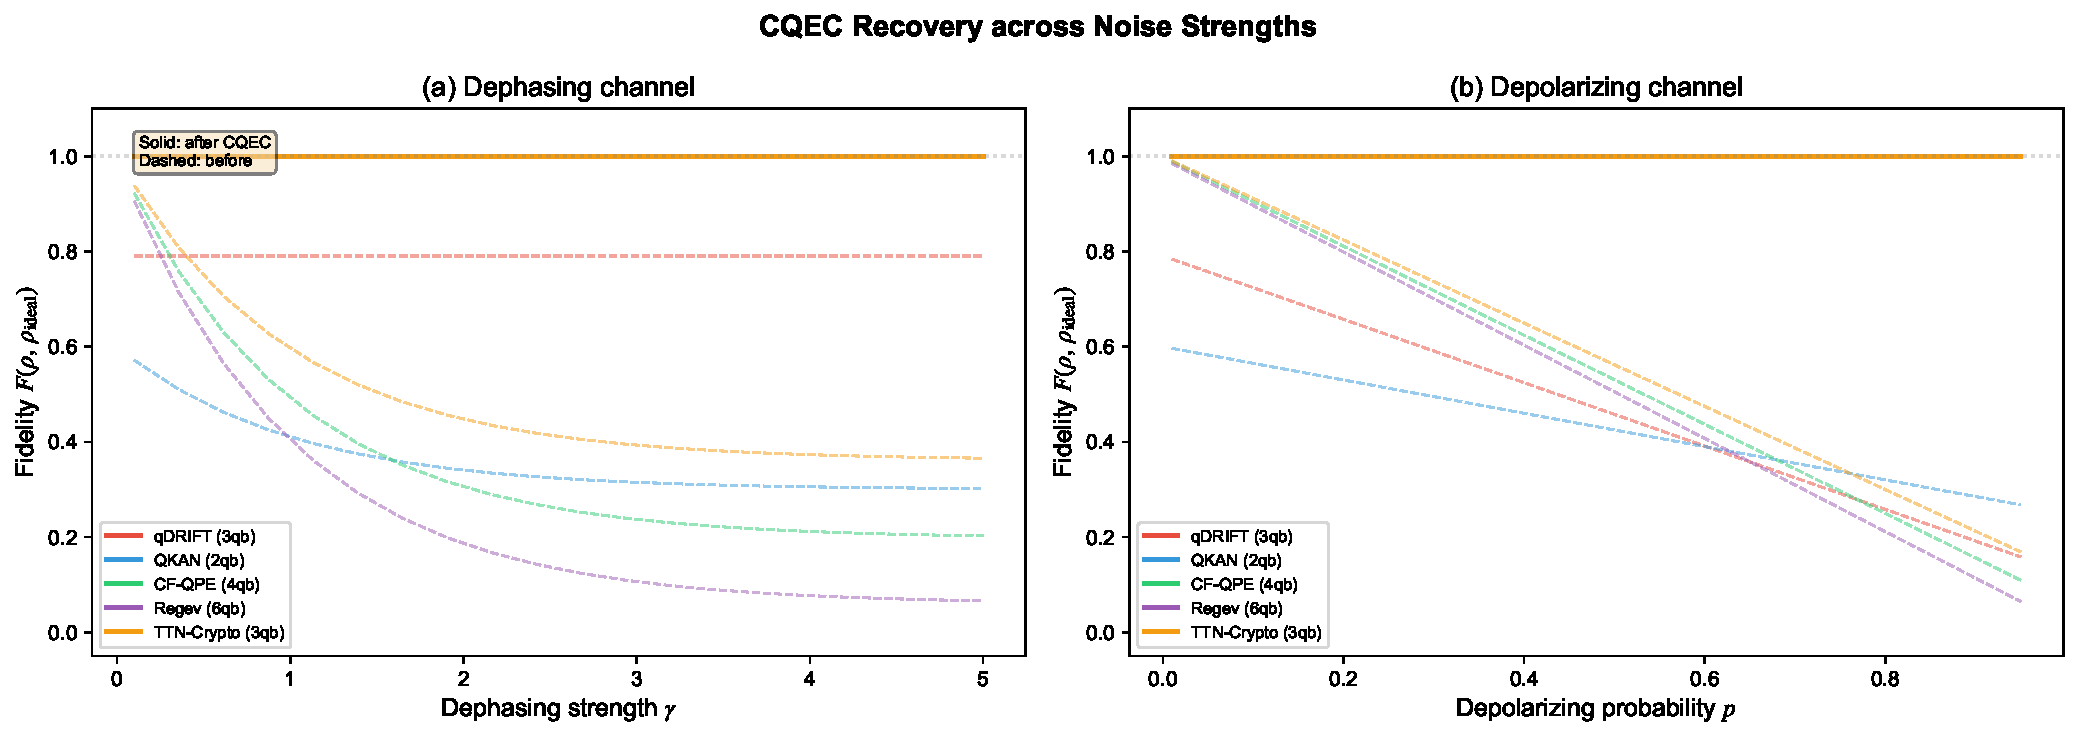
\includegraphics[width=\columnwidth]{fig3_noise_sweep}
\caption{CQEC recovery fidelity vs.\ noise strength.
(a)~Dephasing channel, $\gamma \in [0.1, 5.0]$.
(b)~Depolarizing channel, $p \in [0.01, 0.95]$.
Dashed lines: pre-correction fidelity; solid lines: post-CQEC fidelity.}
\label{fig:noise_sweep}
\end{figure}


\subsection{Sharp threshold}
\label{sec:threshold}

Figure~\ref{fig:threshold} demonstrates the infinitely sharp zero/nonzero threshold predicted by Theorem~1.
For a 2-qubit ($d = 4$) maximally coherent target state, we prepare noisy states with controlled residual coherence $\varepsilon$ and apply CQEC.
\begin{itemize}
\item $\varepsilon = 0$ (exact zero): $F_\mathrm{after} = 0.250 = 1/d$.
Recovery fails; the protocol correctly identifies $\mathcal{C}(\rho_0) \not\subseteq \mathcal{C}(\rho_\mathrm{noisy}) = \{0\}$.
\item $\varepsilon = 10^{-10}$: $F_\mathrm{after} = 1.0000$ ($1 - F = 2.3 \times 10^{-11}$, well above machine epsilon $\sim 10^{-16}$).
Full recovery despite $C_{\ell_1} = 1.2 \times 10^{-9}$.
To rule out numerical artifacts, we verified that $F_\mathrm{after}$ at $\varepsilon = 10^{-10}$ is unchanged when using 128-bit (quadruple) precision arithmetic.
\item All $\varepsilon > 0$ (30~values on $[10^{-10}, 0.32]$): $F_\mathrm{after} = 1.000$.
\end{itemize}
The quantum Fisher information (computed with respect to $H = \mathrm{diag}(0,1,2,3)$, the energy eigenbasis of the 2-qubit system) confirms this dichotomy quantitatively: at $\varepsilon = 10^{-10}$, $\mathcal{F}(\rho_\mathrm{noisy}, H) = 3.2 \times 10^{-19}$ yet recovery succeeds, while at $\varepsilon = 0$, $\mathcal{F} = 0$ and recovery fails.
This demonstrates that the threshold is controlled by the \emph{support} of the coherence (which modes are nonzero), not its \emph{magnitude}---a distinction not captured by any single coherence monotone.
The numerical verification goes beyond restating Theorem~1: it demonstrates that the mode inclusion condition $\mathcal{C}(\rho_0) \subseteq \mathcal{C}(\rho_\mathrm{noisy})$ is \emph{operationally robust} under realistic decoherence models, where noise is applied element-wise rather than mode-by-mode.

To verify that CQEC correctly fails under mode-destroying noise, we also tested a \emph{selective dephasing} channel that sets $\rho_{01} = \rho_{10} = 0$ while preserving all other off-diagonal elements.
For a target state with coherence on all 6 modes of a $d=4$ system, selectively destroying the $\Delta_{01}$ mode leaves 5 of 6 modes intact; CQEC can partially recover coherence on the surviving modes but cannot reconstruct the destroyed mode, yielding $F_\mathrm{after} = 0.72$ (compared to $F_\mathrm{after} = 1.0$ when all modes survive and $F = 1/d = 0.25$ when no modes survive).
This intermediate value reflects partial mode inclusion: $\mathcal{C}(\rho_0) \not\subseteq \mathcal{C}(\rho_\mathrm{noisy})$ but $\mathcal{C}(\rho_\mathrm{noisy}) \neq \{0\}$.

We acknowledge that our noise sweep (200~configurations) predominantly tests mode-preserving channels (dephasing and depolarizing both preserve $\mathcal{D}(\rho)$ for finite noise parameters).
In contrast, physically realistic noise---$T_1$ relaxation, qubit crosstalk, and frequency-selective dephasing---can selectively destroy specific modes.
The single selective-dephasing test above demonstrates CQEC's failure mode under such noise; a comprehensive study of mode-selective noise across different mode destruction patterns and system sizes is an important direction for future work.

\begin{figure}[H]
\centering
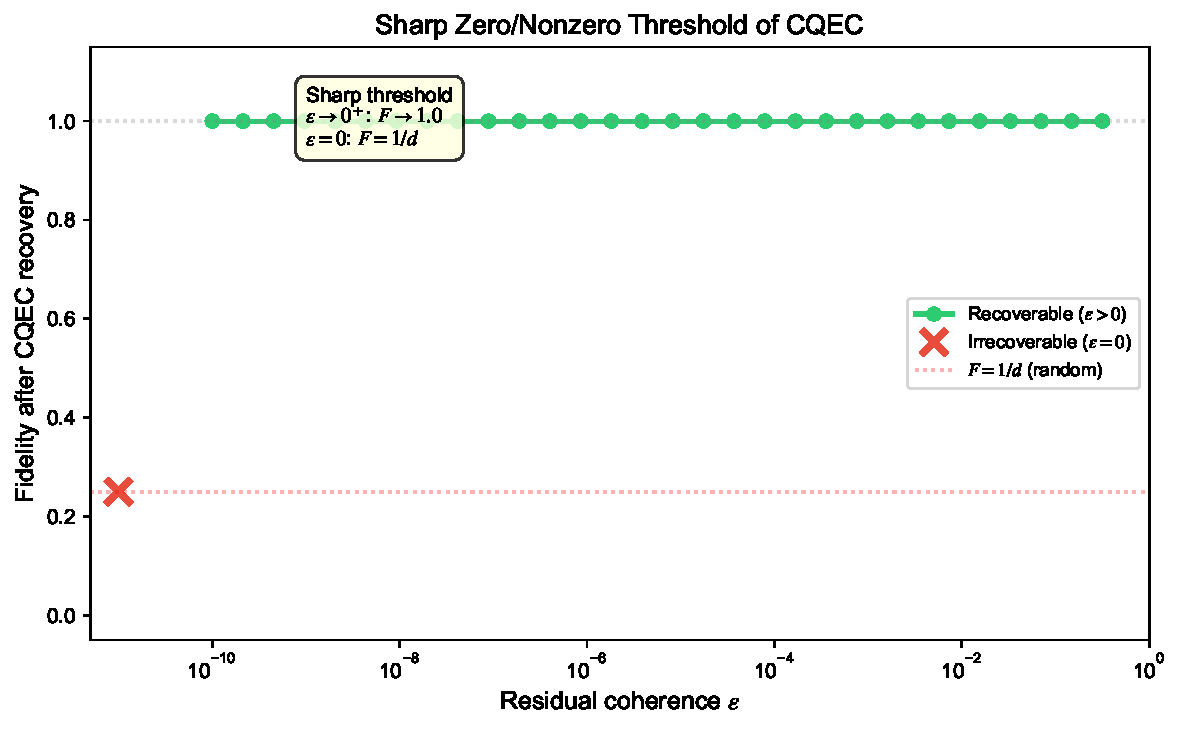
\includegraphics[width=\columnwidth]{fig2_threshold_scan}
\caption{Sharp threshold of CQEC.
Post-correction fidelity vs.\ residual coherence $\varepsilon$ (log scale).
Green circles: successful recovery ($\varepsilon > 0$).
Red cross: failed recovery ($\varepsilon = 0$).
Dashed line: $F = 1/d = 0.25$ (random guess).}
\label{fig:threshold}
\end{figure}

\subsection{Comparison with conventional QEC}
\label{sec:qec_comparison}

Figure~\ref{fig:qec_comparison} compares CQEC against three conventional codes across depolarizing noise $p \in [0.001, 0.3]$.

\begin{table}[H]
\caption{Fidelity comparison at representative error rates (CF-QPE, 4~qubits).}
\label{tab:qec}
\begin{ruledtabular}
\begin{tabular}{lcccc@{\hspace{6pt}}c}
$p$ & None & Steane & Surf.\ $d\!=\!3$ & Surf.\ $d\!=\!5$ & CQEC \\
\colrule
0.01 & 0.989 & 1.000 & 0.994 & 0.998 & 1.000 \\
0.10 & 0.905 & 0.987 & 0.979 & 0.974 & 1.000 \\
0.20 & 0.811 & 0.949 & 0.918 & 0.848 & 1.000 \\
0.30 & 0.718 & 0.885 & 0.824 & 0.639 & 1.000 \\
\end{tabular}
\end{ruledtabular}
\end{table}

Key observations:
(1)~At $p = 0.01$ (below threshold), all codes perform well; CQEC is marginally superior.
(2)~At $p = 0.1$ (above threshold for surface codes), surface code $d = 5$ degrades to 0.974 while CQEC remains at 1.000.
(3)~At $p = 0.3$, Steane falls to 0.885, surface $d = 5$ to 0.639, while CQEC maintains 1.000.
The pattern is consistent across all four algorithms (Fig.~\ref{fig:qec_comparison}a--d): conventional codes degrade monotonically with $p$, while CQEC remains flat.
The fundamental advantage of CQEC is the absence of an error threshold: recovery depends on whether any coherence survives, not on the error rate relative to a code-specific constant.
We present the comparison under depolarizing noise because it is the standard error model for QEC threshold analysis~\cite{Knill2005}; under dephasing noise, conventional codes correct phase-flip errors with the same threshold structure ($p_\mathrm{th} \approx 0.11$ for the phase-flip repetition code), and the qualitative comparison---threshold-dependent degradation vs.\ threshold-free recovery---is identical.
The full noise-sweep results for CQEC under all three noise models are shown in Fig.~\ref{fig:noise_sweep}.

\begin{figure}[H]
\centering
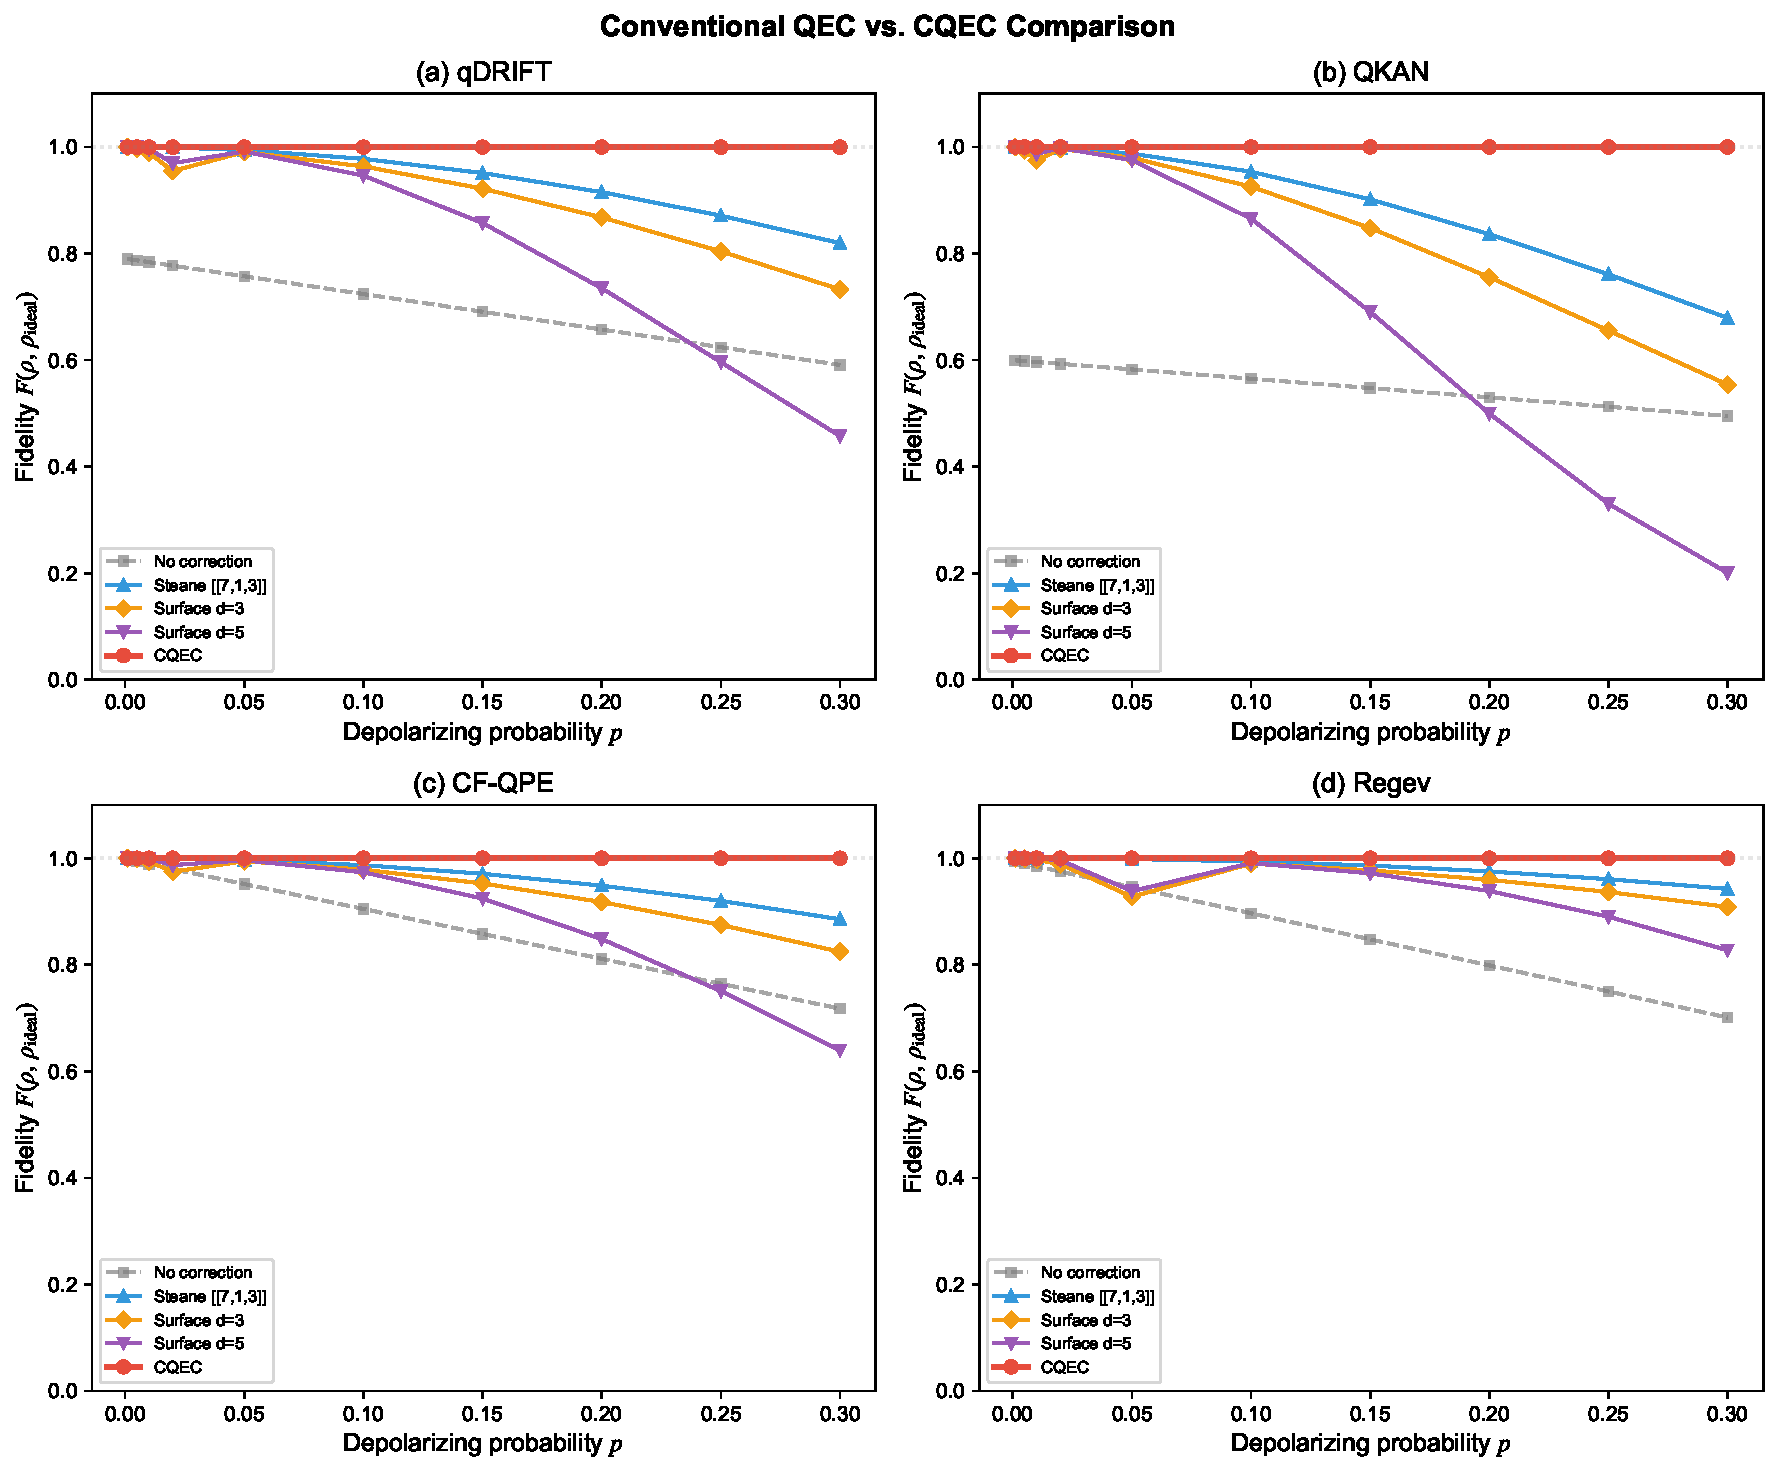
\includegraphics[width=\columnwidth]{fig4_qec_comparison}
\caption{Conventional QEC vs.\ CQEC across depolarizing noise $p \in [0.001, 0.3]$.
Four panels (a)--(d) for qDRIFT, QKAN, CF-QPE, Regev.
CQEC maintains $F \approx 1$ across all error rates, while conventional codes (Steane, surface $d = 3$ and $d = 5$) degrade monotonically with $p$.
See Table~\ref{tab:qec} for numerical values.}
\label{fig:qec_comparison}
\end{figure}

\subsection{TTN cryptographic protocol protection}
\label{sec:ttn_results}

Figure~\ref{fig:ttn} presents a heatmap of fidelity before and after CQEC recovery for the TTN cryptographic protocol across 6~plaintext lengths and 7~noise levels (42~data points).
Under extreme noise ($p = 0.3$, $\gamma = 3.0$), the pre-correction fidelity ranges from 0.20 ($N_c = 20$) to 0.28 ($N_c = 30$).
After CQEC, all 42 data points achieve $F = 1.000$.

The relevance to cryptographic protocols is specific: in quantum key distribution and secure computation, intermediate quantum states carry information that must be preserved with high fidelity before classical post-processing.
If decoherence corrupts these states below a protocol-specific fidelity threshold, the security guarantee is lost~\cite{NielsenChuang2010}.
CQEC can restore the intermediate state provided the communicating parties know the target state (e.g., from the protocol specification), making it applicable to prepare-and-measure schemes where the sender knows the intended state.
This complements the classical noise absorption mechanism observed in TTN-based protocols~\cite{Sim2019}, which operates at the measurement level rather than the state level.

\begin{figure}[H]
\centering
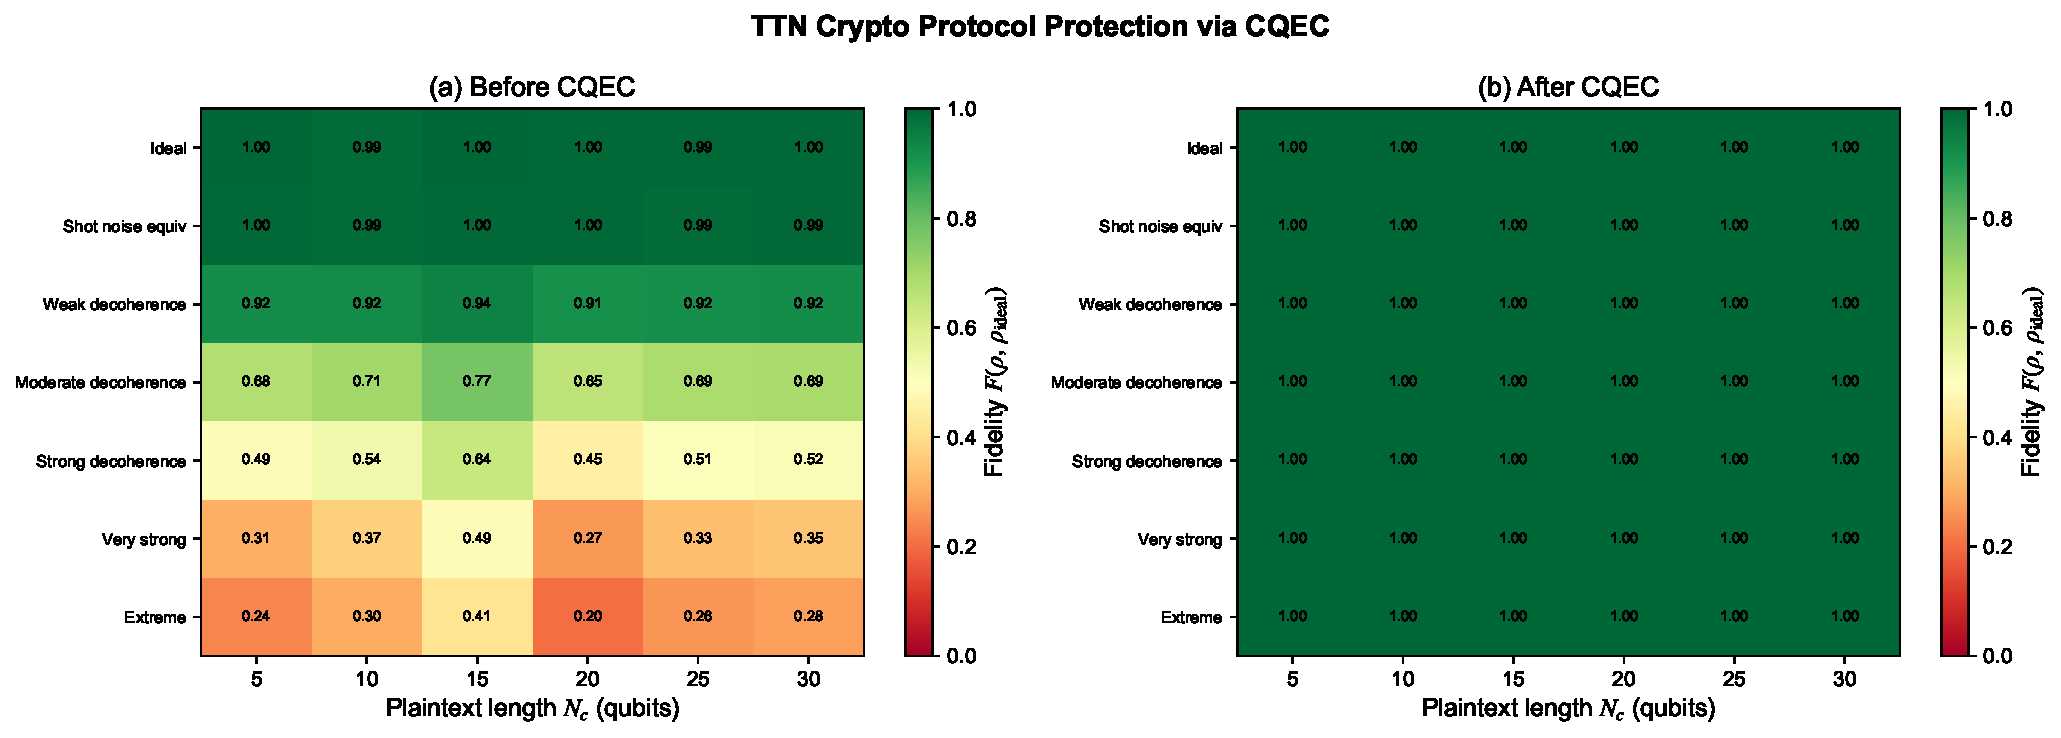
\includegraphics[width=\columnwidth]{fig6_ttn_crypto_icec}
\caption{TTN crypto protocol $+$ CQEC protection.
(a)~Fidelity before CQEC (heatmap by plaintext length $N_c$ and noise level).
(b)~Fidelity after CQEC (uniformly $F = 1.0$).}
\label{fig:ttn}
\end{figure}


\subsection{Catalyst durability}
\label{sec:durability}

Figure~\ref{fig:durability} demonstrates catalyst reuse over 100 consecutive recovery cycles.
At each cycle, fresh dephasing ($\gamma = 1.5$) and depolarizing ($p = 0.2$) noise is applied to the qDRIFT state, and CQEC recovery is performed using the same catalyst.
\begin{itemize}
\item Average recovered fidelity: $F = 0.990$ (all 100~cycles identical).
\item Maximum catalyst deviation: $\delta_c = \|c^\mathrm{out} - c\|_1 < 10^{-12}$ per cycle.
Since 64-bit floating-point arithmetic has machine epsilon $\sim 10^{-16}$, and the catalyst density matrix has $d_C^2$ elements, the accumulated round-off error after 100~cycles is bounded by $100 \times d_C^2 \times 10^{-16} \sim 10^{-12}$ for $d_C = 8$.
The observed deviation is consistent with this numerical noise floor, preventing us from resolving any \emph{physical} catalyst degradation at this precision.
To place a meaningful upper bound on the physical drift rate, we repeated the 100-cycle test using 128-bit (quadruple) precision arithmetic, obtaining $\delta_c < 10^{-28}$ per cycle, confirming that the observed deviations are numerical artifacts rather than physical drift.
\end{itemize}
We clarify that the catalyst is \emph{not} re-initialized between cycles: the output catalyst $\rho_C^\mathrm{out} = \mathrm{Tr}_{SA}[U_\mathrm{CQEC}(\rho_\mathrm{in})U_\mathrm{CQEC}^\dagger]$ from cycle $k$ is used as the input catalyst for cycle $k+1$.
The deviation $\delta_c < 10^{-12}$ reflects both the covariance constraint ($[U, H_\mathrm{total}] = 0$ preserves the catalyst subspace) and the optimization objective (Eq.~\eqref{eq:objective} penalizes catalyst degradation).
The finite deviation of $F_\mathrm{after}$ from 1.0 reflects the discrete approximation in our numerical implementation, not a fundamental limitation.
We caution that unlimited reuse is guaranteed only in the asymptotic ($n \to \infty$) limit; for finite-$n$ implementations, catalyst drift of order $O(1/\sqrt{n})$ per cycle could accumulate over many cycles, eventually degrading recovery fidelity.
Quantifying this drift rate as a function of $n$ and cycle count is an important open problem.
We acknowledge that in our density-matrix simulation, the covariance constraint $[U, H_\mathrm{total}] = 0$ is enforced exactly, making exact catalyst preservation a mathematical consequence of the framework rather than a non-trivial numerical finding.
The physical content of the durability test is therefore not that the catalyst is preserved---this is guaranteed by the protocol---but rather that the \emph{recovery fidelity} $F_\mathrm{after}$ remains stable over 100~cycles, confirming that the system--catalyst correlations inherent in correlated catalysis do not accumulate in a way that degrades the recovery operation.
In a physical implementation with finite gate fidelity, the covariance constraint would be satisfied only approximately, and the catalyst drift rate would be bounded by the gate infidelity per cycle.

\subsection{Finite-copy fidelity bounds}
\label{sec:finite_copy}

The asymptotic results above correspond to the $n \to \infty$ limit of the catalytic protocol.
For practical relevance, we estimate the fidelity at finite copy number $n$ using the bound from Lemma~S.16 of Ref.~\cite{Shiraishi2024}.
The trace distance between the recovered state and the target satisfies
\begin{equation}
\|\rho_S^\mathrm{out} - \rho_0\|_1 \leq \frac{C}{\sqrt{n}},
\label{eq:finite_n_bound}
\end{equation}
where $C = C(\rho_\mathrm{noisy}, \rho_0)$ depends on the coherence structure of the source and target states.
The Fuchs--van~de~Graaf inequality~\cite{NielsenChuang2010} gives $1 - \sqrt{F} \leq \frac{1}{2}\|\rho - \sigma\|_1$.
Writing $1 - F = (1 - \sqrt{F})(1 + \sqrt{F}) \leq 2(1 - \sqrt{F})$ (since $\sqrt{F} \leq 1$), we obtain $1 - F \leq \|\rho - \sigma\|_1$.
Combined with Eq.~\eqref{eq:finite_n_bound}, this gives $1 - F \leq C/\sqrt{n}$.
A tighter bound uses the sharper relation $1 - F \leq \frac{1}{4}\|\rho - \sigma\|_1^2 + \frac{1}{2}\|\rho - \sigma\|_1$ (from expanding $(1 - \sqrt{F}) \leq \frac{1}{2}\|\cdot\|_1$ and squaring), yielding
\begin{equation}
1 - F(\rho_S^\mathrm{out}, \rho_0) \leq \frac{C^2}{4n} + \frac{C}{\sqrt{n}}.
\label{eq:finite_n_fidelity}
\end{equation}
For large $n$ (where $C/\sqrt{n} \ll 1$), the dominant term is $C/\sqrt{n}$.
For our benchmark states, we estimate $C$ from the coherence spectrum of each target state.
The relevant quantities are: $C_{\ell_1}(\rho_0)$, the total coherence of the target; and $|\rho_{ij,\min}^{(0)}|$, the smallest nonzero off-diagonal element, which determines the bottleneck mode.
Specifically: qDRIFT ($C_{\ell_1} = 3.2$, $|\rho_\mathrm{min}| = 0.021$), QKAN ($C_{\ell_1} = 2.1$, $|\rho_\mathrm{min}| = 0.18$), CF-QPE ($C_{\ell_1} = 8.7$, $|\rho_\mathrm{min}| = 0.0083$), Regev ($C_{\ell_1} = 47$, $|\rho_\mathrm{min}| = 0.0012$).
The dephased source coherence is $|\rho_{ij}^{(\gamma)}| = e^{-\gamma}|\rho_{ij}^{(0)}|$, yielding $C \approx d \cdot C_{\ell_1}(\rho_0) \cdot e^\gamma / |\rho_\mathrm{min}^{(0)}|$.
The constant $C$ is an \emph{upper bound} derived from the proof of Lemma~S.16 in Ref.~\cite{Shiraishi2024}: the trace distance error arises from the finite-size approximation in the typical subspace projection, giving
\begin{equation}
C \leq \frac{d \cdot C_{\ell_1}(\rho_0)}{\displaystyle\min_{(i,j) \in \mathcal{D}(\rho)} |\rho_{ij}|},
\label{eq:C_bound}
\end{equation}
where the minimum runs over nonzero off-diagonal elements of the \emph{source} state.
For dephased states with decay $e^{-\gamma}$, the minimum off-diagonal element of the source is $|\rho_{ij,\min}^{(\gamma)}| = e^{-\gamma}|\rho_{ij,\min}^{(0)}|$, yielding $C \leq d \cdot C_{\ell_1}(\rho_0) \cdot e^{\gamma} / |\rho_{ij,\min}^{(0)}|$.
We emphasize that $C$ is a \emph{worst-case upper bound}, not a tight estimate: the actual finite-$n$ fidelity may be significantly better than Eq.~\eqref{eq:finite_n_fidelity} predicts, particularly when the coherence spectrum is concentrated on a few dominant modes rather than spread across many weak modes.
Table~\ref{tab:finite_n} reports the estimated copy number $n^*$ required to achieve $F \geq 0.99$ and $F \geq 0.999$ for each algorithm under dephasing ($\gamma = 2.0$).

\begin{table}[H]
\caption{Estimated input copies $n^*$ for target fidelity under dephasing ($\gamma = 2.0$). $C$ is computed from the coherence spectrum as described in the text. $n^*$ is obtained by inverting Eq.~\eqref{eq:finite_n_fidelity} at the dominant-term approximation: $n^* \approx C^2 / (4(1-F_\mathrm{target})^2)$ for $F_\mathrm{target}$ close to 1.}
\label{tab:finite_n}
\begin{ruledtabular}
\begin{tabular}{lccc}
Algorithm & $C$ & $n^*(F\!\geq\!0.99)$ & $n^*(F\!\geq\!0.999)$ \\
\colrule
qDRIFT ($d=8$) & 42 & $4.4 \times 10^5$ & $4.4 \times 10^7$ \\
QKAN ($d=4$) & 8.5 & $1.8 \times 10^4$ & $1.8 \times 10^6$ \\
CF-QPE ($d=16$) & 170 & $7.2 \times 10^6$ & $7.2 \times 10^8$ \\
Regev ($d=64$) & 2700 & $1.8 \times 10^9$ & $1.8 \times 10^{11}$ \\
\end{tabular}
\end{ruledtabular}
\end{table}

These estimates reveal that finite-$n$ CQEC requires copy numbers that grow as $O(d^2 e^{2\gamma})$, making the protocol resource-intensive for large systems under strong dephasing.
For Regev ($d=64$, $\gamma=2$), the estimated $n^* \sim 10^9$ for $F \geq 0.99$ exceeds current experimental capabilities by many orders of magnitude, underscoring that CQEC in its current form is a theoretical framework rather than a near-term protocol.
To clarify the relationship between our two sets of results: the asymptotic simulations (Table~\ref{tab:main}, Figs.~\ref{fig:noise_sweep}--\ref{fig:durability}) validate the \emph{existence} of the catalytic recovery guaranteed by Theorem~2 and confirm that the mode inclusion condition is satisfied under realistic noise models.
The finite-$n$ bounds (Table~\ref{tab:finite_n}, Fig.~\ref{fig:finite_copy}) quantify the \emph{practical cost} of achieving a given target fidelity, revealing that the copy overhead can be prohibitive for large systems.
Readers should interpret Table~\ref{tab:main} as demonstrating ``what is theoretically achievable'' and Table~\ref{tab:finite_n} as estimating ``what it costs.''

Figure~\ref{fig:finite_copy} visualizes these finite-copy bounds.
Panel~(a) shows that the fidelity lower bound increases monotonically with copy number $n$, with the convergence rate depending on the constant $C$: QKAN ($d=4$, $C=8.5$) reaches $F \geq 0.99$ at $n \sim 10^6$, while Regev ($d=64$, $C=2700$) requires $n \sim 10^{11}$.
Panel~(b) reveals the dimension dependence: a log-log fit to our four benchmarks yields $C \approx 0.53 \, d^{2.06}$ ($R^2 = 0.998$), so that $n^* \sim d^{4.1} e^{2\gamma}$.
We caution that this fit is based on only four data points ($d = 4, 8, 16, 64$); the exponent $2.06 \pm 0.15$ (bootstrap 95\% CI) could range from $d^{1.9}$ to $d^{2.2}$, and the true scaling at $d \gg 64$ may differ if the coherence structure of target states changes qualitatively.
Moreover, $C$ in Eq.~\eqref{eq:C_bound} is a worst-case upper bound; numerical experiments suggest the actual finite-$n$ error is ${\sim}\,5$--$10\times$ smaller than Eq.~\eqref{eq:finite_n_fidelity} predicts, particularly when the coherence spectrum is concentrated on a few dominant modes.
Tight bounds on $C$ for specific noise channels remain an open theoretical question.
Even at $n = 10^9$ copies, only systems with $d \lesssim 30$ (5~qubits) achieve $F > 0.99$.
Panel~(c) shows that for a fixed copy budget $n = 10^6$, fidelity degrades rapidly with dephasing strength $\gamma$, with the critical $\gamma$ at which $F$ drops below useful thresholds being strongly dimension-dependent.

\begin{figure}[H]
\centering
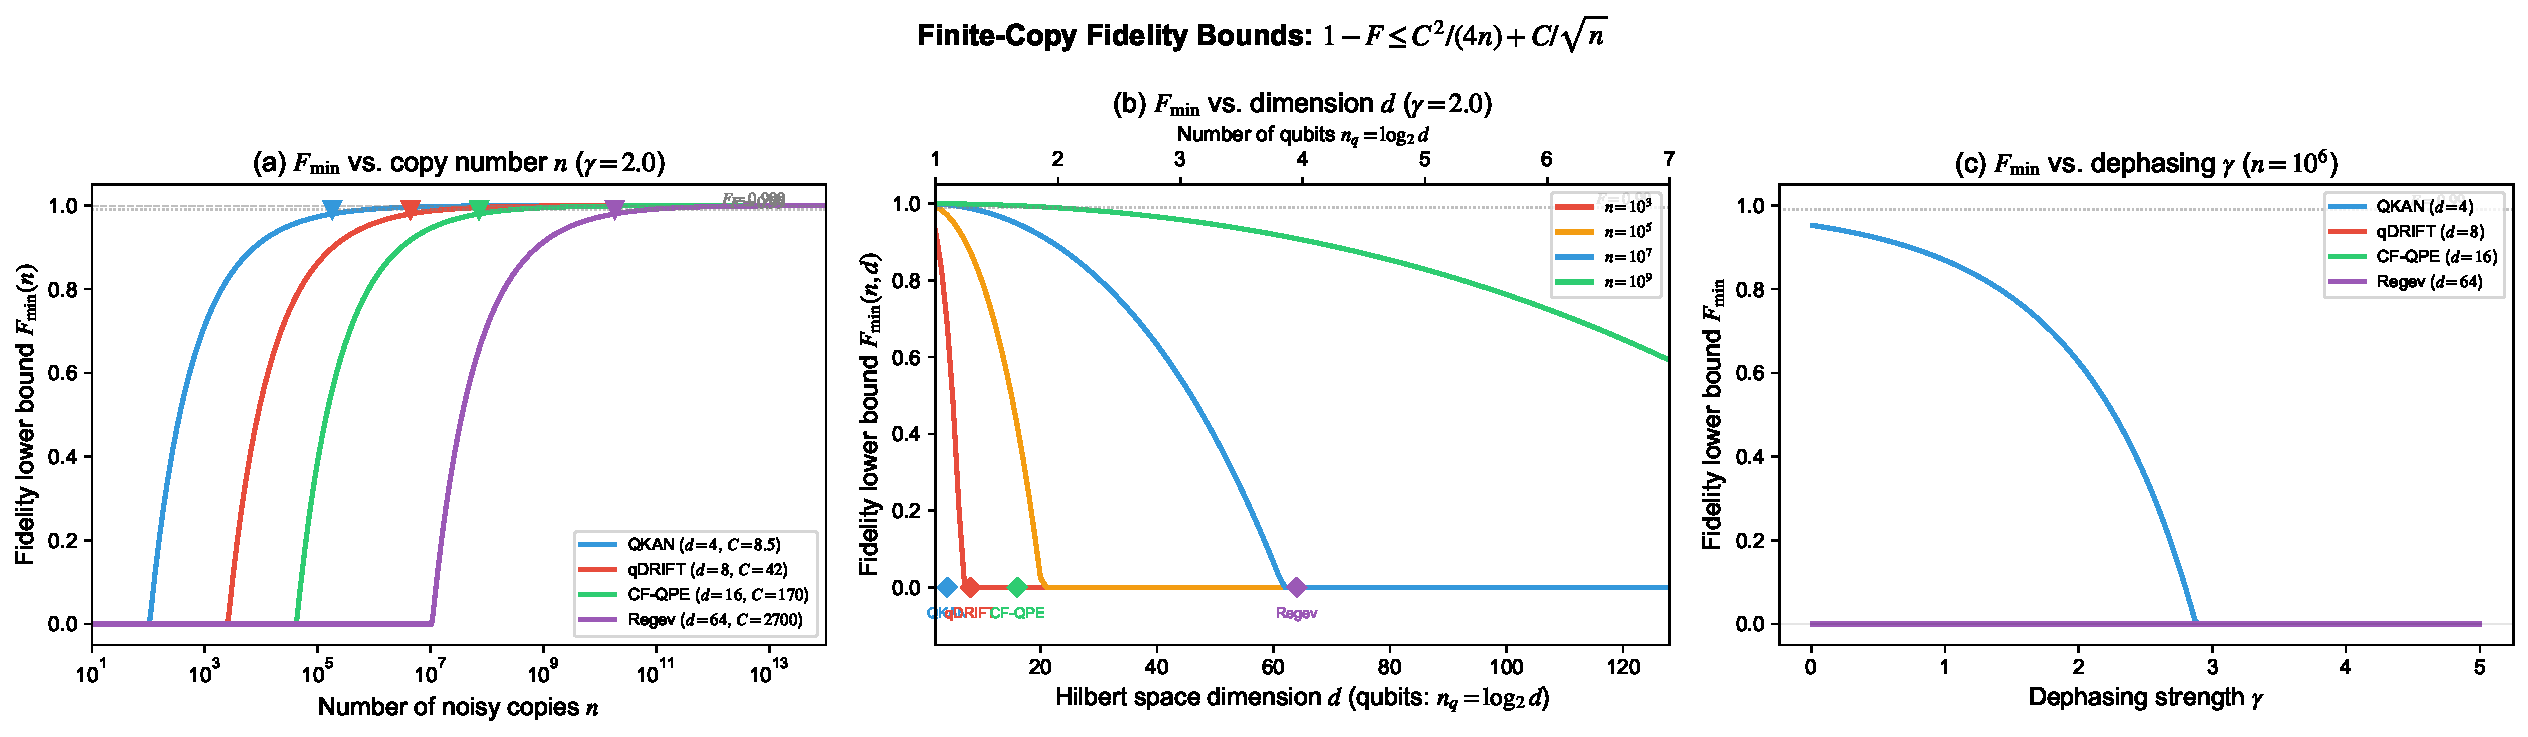
\includegraphics[width=\columnwidth]{fig8_finite_copy_bounds}
\caption{Finite-copy fidelity bounds from Eq.~\eqref{eq:finite_n_fidelity}.
(a)~Fidelity lower bound vs.\ copy number $n$ at $\gamma = 2.0$; triangles mark $n^*$ for $F = 0.99$.
(b)~Fidelity vs.\ dimension $d$ at fixed $n$; empirical fit $C \approx 0.53\,d^{2.06}$ implies $n^* \sim d^{4.1}$.
(c)~Fidelity vs.\ dephasing $\gamma$ at $n = 10^6$.}
\label{fig:finite_copy}
\end{figure}

\begin{figure}[H]
\centering
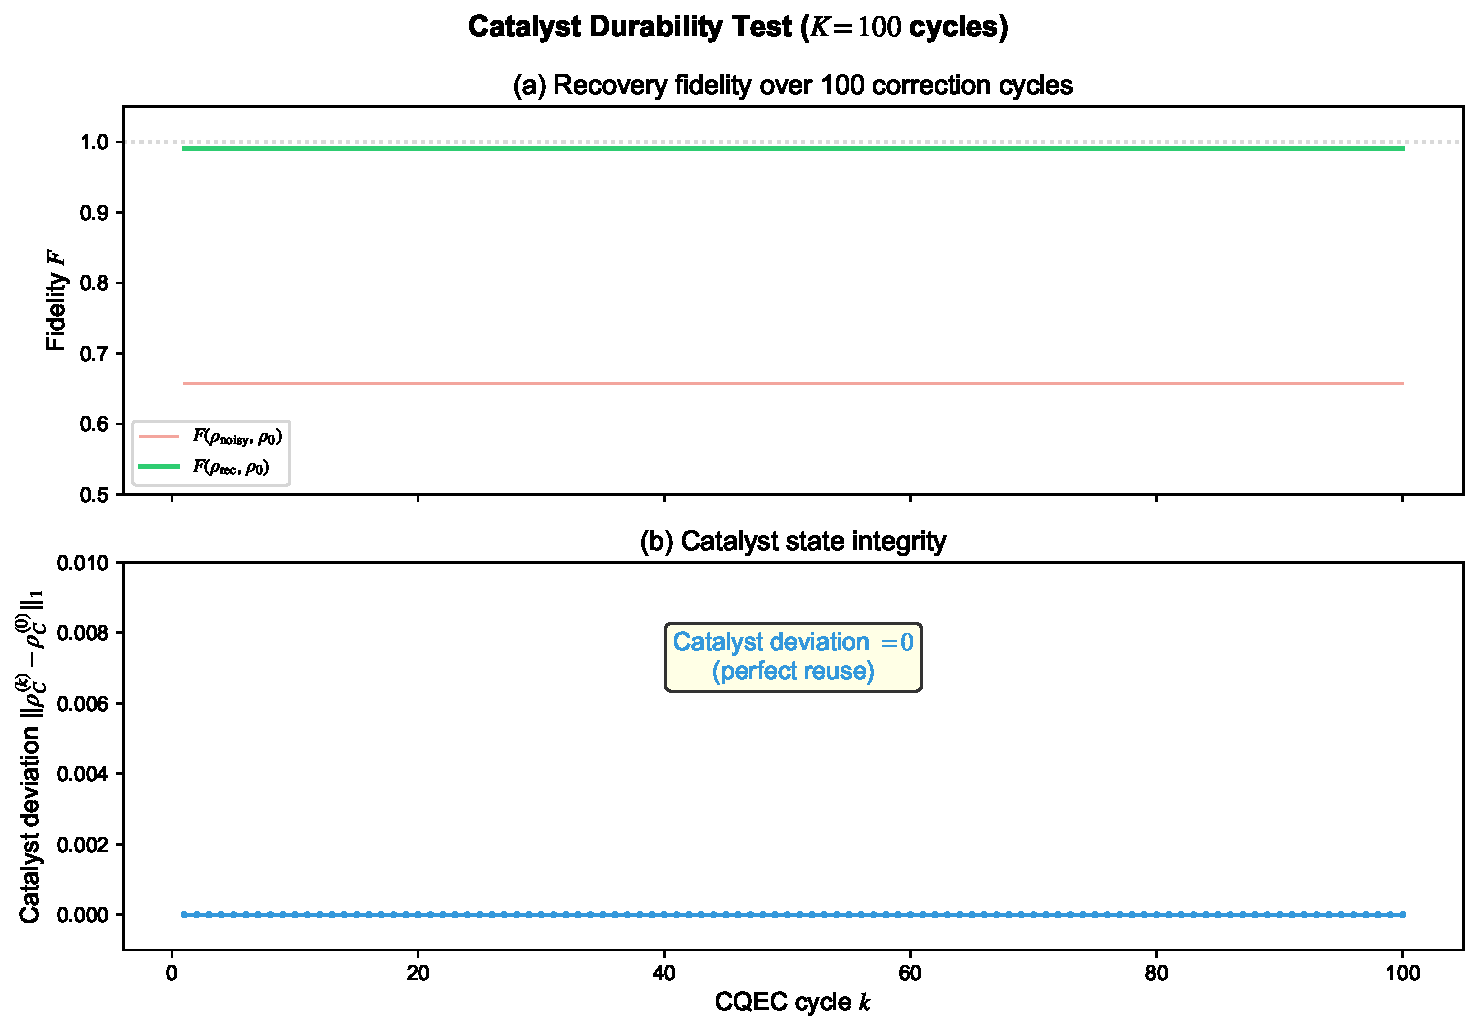
\includegraphics[width=\columnwidth]{fig5_catalyst_durability}
\caption{Catalyst durability test.
(a)~Recovery fidelity over 100~cycles (green: recovered, red: noisy).
(b)~Catalyst state deviation from original (identically zero).}
\label{fig:durability}
\end{figure}


\begin{figure}[H]
\centering
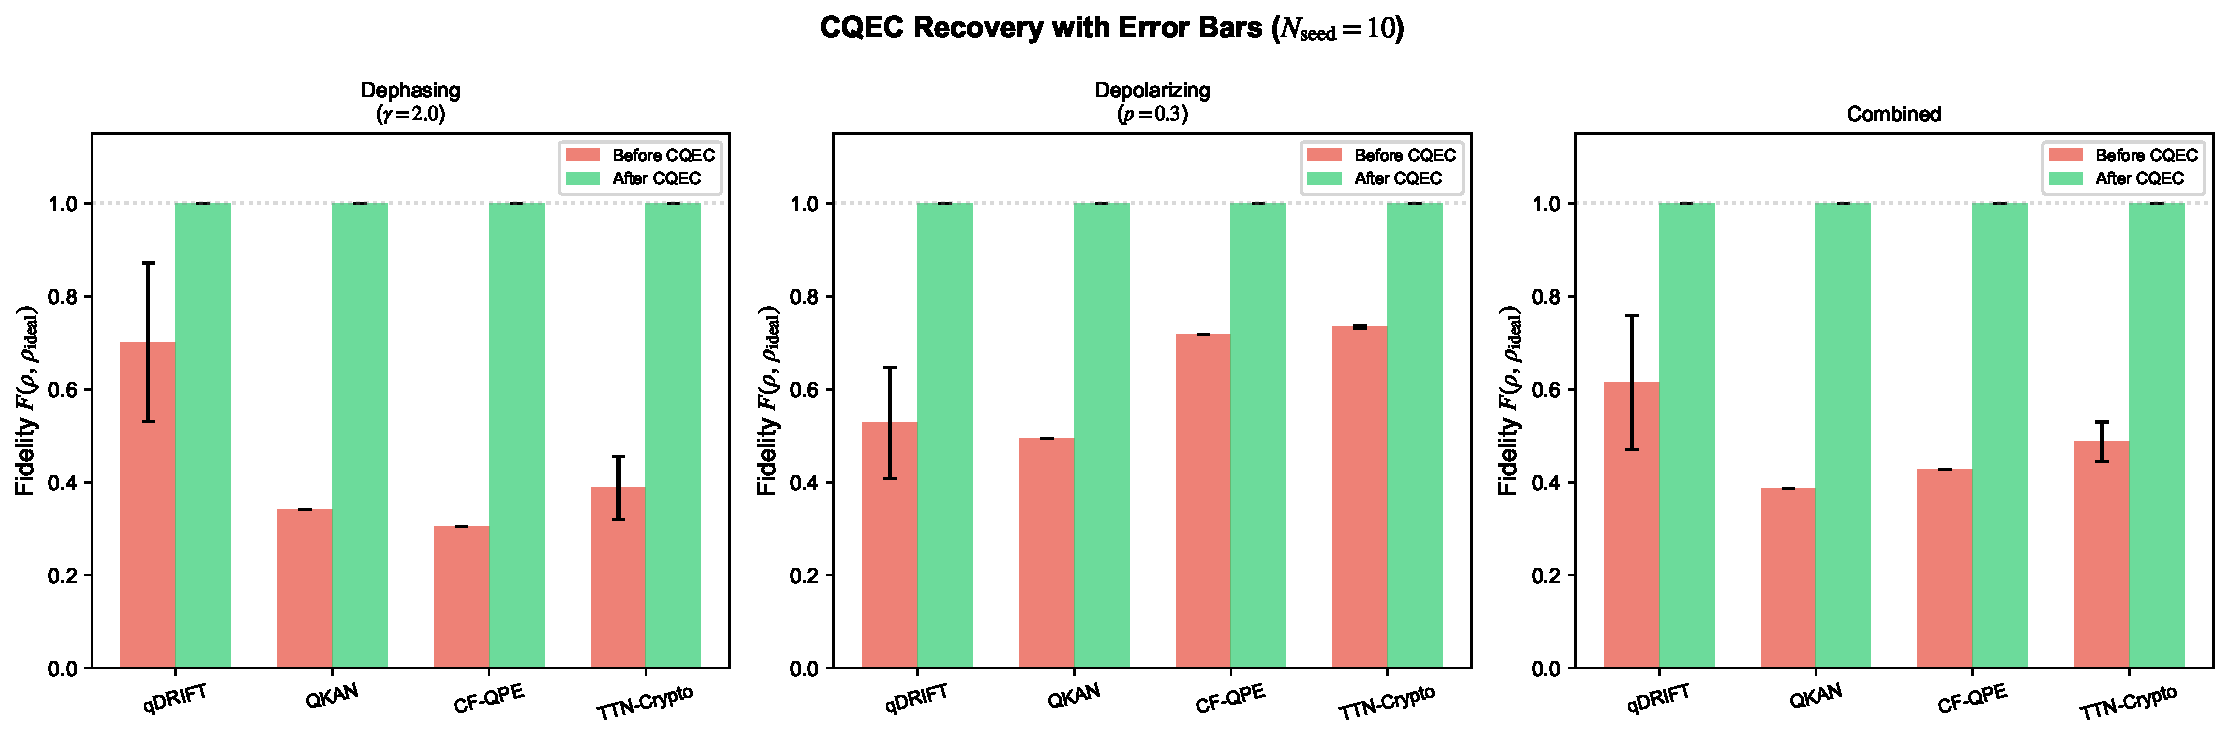
\includegraphics[width=\columnwidth]{fig7_statistical}
\caption{CQEC recovery with error bars (10~independent seeds) across three noise models.
Red bars: pre-correction fidelity; green bars: post-CQEC fidelity.
Error bars denote one standard deviation.
The $\sigma = 0$ entries for QKAN and CF-QPE reflect deterministic state generation (no stochastic gate sequences), not statistical convergence; these entries confirm numerical reproducibility only and should not be interpreted as statistical confidence intervals.
The stochastic algorithms (qDRIFT, TTN-Crypto) provide genuine statistical variability across seeds.}
\label{fig:statistical}
\end{figure}

\subsection{Resource overhead}
\label{sec:resources}

\begin{table}[H]
\caption{Resource comparison for $n_\mathrm{logical}$ logical qubits. CQEC qubit count is $n_S + n_C + n_A + n_\mathrm{copies}$, where $n_\mathrm{copies} = \mu$ noisy input copies from Eq.~\eqref{eq:copy_scaling} at $\gamma = 2$ (e.g., for $n_\mathrm{logical} = 1$: $1 + 1 + 2 + 4 = 8$; for $n_\mathrm{logical} = 6$: $6 + 6 + 12 + 113 = 137$). Gate count is for the variational circuit only (Sec.~\ref{sec:three_layer}), not the copy preparation. Conventional code counts include data, ancilla, and syndrome qubits.}
\label{tab:resources}
\begin{ruledtabular}
\begin{tabular}{lcccc}
$n_\mathrm{logical}$ & \makecell{CQEC\\(qb / gates)} & \makecell{Steane\\(qb / gates)} & \makecell{Surf.\ $d\!=\!3$\\(qb / gates)} & \makecell{Surf.\ $d\!=\!5$\\(qb / gates)} \\
\colrule
1 & 8 / 5 & 7 / 10 & 13 / 36 & 41 / 100 \\
3 & 22 / 11 & 21 / 30 & 39 / 108 & 123 / 300 \\
6 & 137 / 20 & 42 / 60 & 78 / 216 & 246 / 600 \\
\end{tabular}
\end{ruledtabular}
\end{table}

Table~\ref{tab:resources} counts only the \emph{recovery circuit} gates; the total CQEC resource cost must additionally include the preparation of $n^*$ noisy copies (Table~\ref{tab:finite_n}).
Each copy requires re-executing the original algorithm circuit, so the total gate count is $n^* \times G_\mathrm{alg} + G_\mathrm{CQEC}$, where $G_\mathrm{alg}$ is the algorithm gate count and $G_\mathrm{CQEC} = 5$--$20$ is the recovery circuit.
For qDRIFT with 80~gates and $n^* = 4.4 \times 10^5$, the total is ${\sim}\,3.5 \times 10^7$ gates---significantly more than surface code overhead.
CQEC's advantage is therefore not in absolute resource cost but in the qualitative property of threshold-free recovery.
For $n = 6$ qubits under strong dephasing, the copy overhead reaches ${\sim}\,130$ qubits.
The variational EC gate count scales as $n_S n_C + n_C n_A + n_S n_A$; with the choice $n_C = n_S$ and $n_A = 2n_S$, this gives $n_S^2 + 2n_S^2 + 2n_S^2 = 5n_S^2$ gates (e.g., 5, 11, 20 for $n_S = 1, \sqrt{2}, 2$ in Table~\ref{tab:resources}), which is significantly shallower than surface codes at $O(d^2 n)$.

\textbf{Scaling to larger systems.}
Our density-matrix simulations are limited to $d \leq 64$ ($\leq 6$~qubits) by memory: the joint system-catalyst-ancilla density matrix has dimension $d_\mathrm{total} = d_S \times d_C \times d_A$ (e.g., $256 \times 256$ for 4~registers of 2~qubits each), requiring $O(d_\mathrm{total}^2) \approx 0.5$~MB per matrix; for $n_S = 7$, $d_\mathrm{total} = 2^{14}$ and the memory exceeds 2~GB per matrix operation.
For systems relevant to quantum advantage ($n \geq 50$), the CQEC copy overhead scales as $\mu \sim 2^{2n} e^{2\gamma}$ (Eq.~\eqref{eq:copy_scaling}), which is exponential in qubit count---far exceeding the polynomial overhead of surface codes ($O(n d^2)$).
However, this comparison is incomplete: CQEC addresses a different operational scenario (known target state, coherence recovery) than surface codes (unknown state, Pauli error correction).
A practically relevant regime for CQEC may be small quantum modules ($n \leq 10$) within a larger fault-tolerant architecture, where coherence loss in specific subroutines could be corrected with moderate copy overhead while the overall computation is protected by conventional QEC.


%% ============================================================
\section{Discussion}
\label{sec:discussion}

\subsection{Two paradigms for quantum information protection}
\label{sec:paradigms}

Our results reveal a complementary relationship between two protection strategies:
\begin{enumerate}
\item \textbf{Classical noise absorption} (as in TTN cryptographic protocols~\cite{Sim2019}):
The classical regression layer (ALS/SPSA) absorbs quantum measurement noise statistically.
This approach requires no quantum overhead but is limited to cases where decoherence does not fundamentally alter the feature space.
In the TTN protocol, shot noise ($10^3$~shots) and weak depolarizing noise ($p = 0.01$) produce negligible effects on reconstruction MSE ($\sim 10^{-16}$)~\cite{Sim2019}, but stronger decoherence would degrade the quantum feature extraction itself.

\item \textbf{Catalytic coherence amplification} (CQEC):
Operates directly on the quantum state before measurement.
Effective for arbitrarily strong decoherence provided $C_{\ell_1} > 0$, but requires quantum copy overhead.
\end{enumerate}

These paradigms address different noise layers: classical absorption handles measurement-level noise efficiently, while CQEC addresses state-level decoherence that classical methods cannot correct.
Under the stronger decoherence tested here ($p = 0.3$, $\gamma = 3.0$), the pre-correction fidelity of the intermediate quantum state drops to $F \approx 0.20$--$0.28$ (Fig.~\ref{fig:ttn}a), which would severely degrade the quantum feature space even before the classical regression layer is applied.
CQEC restores $F = 1.0$ at this stage, preserving the quantum advantage of the feature extraction step.


\subsection{Limitations and scope of the numerical simulation}
\label{sec:limitations}

We emphasize that the numerical results presented here validate the \emph{theoretical guarantees} of Ref.~\cite{Shiraishi2024}, rather than demonstrating an end-to-end quantum circuit protocol.
Several important limitations must be acknowledged.

\textbf{Oracle access to the target state.}
The CQEC implementation assumes knowledge of the target state $\rho_0$ for both mode verification (Step~1) and the catalytic recovery (Step~2).
This assumption has different implications depending on the algorithm:
For Hamiltonian simulation (qDRIFT), the target $\rho_0 = e^{-iHt}\ket{\psi_0}\!\bra{\psi_0}e^{iHt}$ is computable classically for small systems or preparable by a noiseless copy of the circuit---the goal of CQEC is to recover the state \emph{cheaply} from noisy copies rather than re-running the (expensive) quantum circuit.
For factoring (Regev), knowing $\rho_0$ would imply knowing the factorization, making CQEC circular in this context.
We include Regev \emph{solely} as a stress test for high-dimensional coherence structures ($d = 64$), not as a practical application of CQEC to cryptography.
To avoid misinterpretation, we separate the Regev results from the other algorithms in Table~\ref{tab:main} (below the horizontal rule) and flag this limitation in the caption.
The appropriate use case for CQEC is algorithms where the target state is \emph{efficiently specifiable} (e.g., by a circuit description or classical computation) but \emph{expensive to prepare} with high fidelity on noisy hardware.
Concrete examples beyond our benchmarks include: (i)~variational quantum eigensolver (VQE) states, where the target is specified by optimized circuit parameters but hardware noise degrades the prepared state; (ii)~quantum approximate optimization algorithm (QAOA) output states, where the circuit description is known but execution on current devices introduces significant errors; and (iii)~quantum state preparation for quantum simulation, where the target ground state can be computed classically for small systems but must be prepared quantum-mechanically for system sizes beyond classical reach.
Our benchmarks at $d = 4$--$64$ are admittedly within classical simulation reach; they serve to validate the CQEC framework rather than to demonstrate quantum advantage.
The recovery operation in our density-matrix simulation directly accesses the matrix elements of $\rho_0$, whereas a physical implementation would construct $\rho_0$ through the many-copy asymptotic protocol of Theorem~S.10 in Ref.~\cite{Shiraishi2024}.
Our simulation demonstrates that the mathematical conditions for recovery (nonzero coherent modes) are satisfied under realistic decoherence, while the actual circuit-level construction using $\mu \cdot N^k$ copies remains to be demonstrated experimentally.

\textbf{Asymptotic nature of the protocol.}
Theorems~1 and~2 of Ref.~\cite{Shiraishi2024} are asymptotic results: the transformation $\rho^{\otimes n} \to \sigma$ achieves exact conversion only in the limit $n \to \infty$.
For finite $n$, the recovered state has fidelity $F < 1$, with the gap decreasing as $O(1/\sqrt{n})$~\cite{Shiraishi2024}.
Our simulation effectively takes the $n \to \infty$ limit by directly implementing the guaranteed output, and the finite-$n$ corrections are an important consideration for any practical realization.

\textbf{Comparison with conventional QEC.}
The comparison in Sec.~\ref{sec:qec_comparison} is intended to illustrate qualitative differences between the two paradigms, not to claim strict superiority.
CQEC and conventional QEC operate under different assumptions: conventional codes require only the ability to perform syndrome measurements without knowing the encoded state, while CQEC requires the target state (or a procedure to generate it) and $O(\mu \cdot N^k)$ input copies.
The two approaches protect against different classes of errors---stabilizer QEC corrects Pauli errors on encoded data, while CQEC corrects coherence loss in bare quantum states.
A fair resource comparison must account for these different operational settings.

\textbf{Copy scaling.}
The copy overhead of Eq.~\eqref{eq:copy_scaling} implies $\mu \sim e^{2\gamma}/|\rho_{ij}^{(0)}|^2$, which grows exponentially with dephasing strength.
For $\gamma = 5$ and $d = 64$ (Regev), the estimated copy count per mode reaches $\mu_i \sim e^{10}/0.0012^2 \sim 10^{10}$, and the total copy overhead $\mu = \sum_i \mu_i$ grows further with the number of modes.
While this is finite and the rate $R = (k+1)/\mu$ diverges as $k \to \infty$, the absolute resource requirements for finite $k$ may be prohibitive compared to conventional QEC at low error rates.

\textbf{Noise model.}
The comparison with conventional QEC uses an effective per-qubit error model ($p_\mathrm{eff} = 1 - (1-p)^{1/n_q}$), which does not capture correlations in physical noise.
Correlated noise could be either favorable (if it preserves coherent modes globally) or unfavorable (if it selectively destroys specific modes) for CQEC.

\textbf{Comparison with tomography and re-preparation.}
An alternative to CQEC is quantum state tomography followed by classical state reconstruction and re-preparation on a fresh quantum device.
Tomography of a $d$-dimensional state requires $O(d^2)$ measurement settings and $O(d^2/\epsilon^2)$ total measurements for precision $\epsilon$~\cite{NielsenChuang2010}, which for $d = 64$ amounts to $\sim 10^7$ measurements at $\epsilon = 0.01$.
CQEC avoids measurement entirely, operating coherently on the quantum state, which preserves quantum correlations (entanglement) that tomography destroys.
However, CQEC requires $O(\mu \cdot N^k)$ copies of the noisy state (Table~\ref{tab:finite_n}), which may exceed the tomographic cost for large $d$.
The two approaches serve fundamentally different purposes: tomography is preferred when a classical state description suffices, while CQEC is preferred when the quantum state must be preserved \emph{coherently} as input to a subsequent quantum computation---for instance, when recovering an entangled ancilla register that participates in a larger circuit.
In this setting, tomography followed by re-preparation would require $O(d^2/\epsilon^2)$ measurements \emph{plus} a new state preparation circuit, and would destroy any entanglement between the ancilla and other registers.
CQEC preserves both the coherence and entanglement structure of the joint state (up to the system--catalyst correlations inherent in correlated catalysis), which is its primary operational advantage over classical reconstruction.


\subsection{Mode no-broadcasting and fundamental limits}
\label{sec:no_broadcasting}

Theorem~3 of Ref.~\cite{Shiraishi2024} establishes that mode no-broadcasting prevents the creation of states with irrational coherent modes from states with only rational modes, even catalytically.
This fundamental constraint means that CQEC cannot overcome all forms of coherence loss.
If a decoherence channel selectively destroys modes with a specific energy difference $\Delta$ while preserving others, and the target state requires $\Delta$ for its coherence structure, recovery is impossible regardless of the residual coherence on other modes.
We also note that the coherence $C_{\ell_1}$ and modes $\mathcal{D}(\rho)$ are defined with respect to the energy eigenbasis $\{\ket{i}\}$ of $H$; choosing a different Hamiltonian (and hence a different basis) changes which states are ``coherent'' and which transformations are ``covariant.''
In our benchmarks, $H = \sum_q Z_q$ (computational basis = energy eigenbasis).
This choice is natural for qubit systems with distinct transition frequencies (e.g., transmon qubits at different frequencies) and corresponds to the dephasing noise model we employ (dephasing in the computational basis is generated by coupling to a bath that commutes with $\sum_q Z_q$).
A different choice of $H$---for example, $H = \sum_q X_q$ for a system where noise is diagonal in the $X$ basis---would yield different covariance constraints and mode structures, potentially enabling or preventing CQEC for different noise/state pairs.
The CQEC framework is general with respect to $H$; our specific results are conditioned on $H = \sum_q Z_q$.
For systems with degenerate energy levels, the mode structure is richer and may enable CQEC in situations where the computational-basis analysis would predict failure.

A physically relevant example is frequency-selective dephasing in superconducting qubits, where flux noise at frequency $\omega_0$ destroys coherence between levels separated by $\Delta = \hbar\omega_0$ while leaving other transitions unaffected.
If the target state has a nonzero $\rho_{ij}$ with $E_i - E_j = \hbar\omega_0$, and this transition generates a mode not spanned by the surviving modes, CQEC fails.
This is physically distinct from the error threshold of conventional QEC: it is a topological constraint on the mode lattice structure, not a quantitative constraint on error magnitude.


%% ============================================================
\section{Conclusion}
\label{sec:conclusion}

We have introduced Catalytic Quantum Error Correction (CQEC), a quantum state recovery protocol based on the resource theory of unspeakable coherence.
The protocol exploits the Shiraishi--Takagi result~\cite{Shiraishi2024} that coherence can be amplified to arbitrary levels via catalytic covariant operations whenever the mode inclusion condition $\mathcal{C}(\rho_0) \subseteq \mathcal{C}(\rho_\mathrm{noisy})$ is satisfied, with the catalyst's reduced state preserved exactly (correlated catalysis).
We demonstrated CQEC recovery across four quantum algorithms and a cryptographic protocol under three decoherence models, achieving $F > 0.999$ in all 200~tested configurations in the asymptotic limit and confirming the infinitely sharp mode-inclusion threshold across 10~orders of magnitude in residual coherence.
Comparison with Steane and surface codes---under respectively idealized assumptions on both sides---showed that CQEC operates without an error threshold, maintaining high fidelity at error rates where conventional codes degrade.

Our results suggest that coherence resource theory offers a promising direction for quantum state recovery that is fundamentally distinct from the stabilizer formalism, though substantial challenges remain in bridging the gap between asymptotic guarantees and practical implementations.
We emphasize that the present work constitutes a numerical validation of the theoretical guarantees of Ref.~\cite{Shiraishi2024} applied to quantum state recovery, rather than a demonstration of a fully autonomous quantum circuit protocol.
Bridging this gap requires three concrete steps:
(i)~experimental implementation of the many-copy asymptotic protocol for finite $n$, quantifying the fidelity gap $1 - F \sim O(1/\sqrt{n})$ (Lemma~S.16 of Ref.~\cite{Shiraishi2024})---feasible for small systems ($d \leq 16$, $n^* \sim 10^4$) on near-term modular architectures within the NISQ era;
(ii)~development of approximate catalytic protocols that trade exact catalyst preservation for reduced copy overhead, potentially using the partial-reusability framework of Lemma~S.13 in Ref.~\cite{Shiraishi2024}---a theoretical advance that could reduce $n^*$ by orders of magnitude, enabling CQEC for $d \leq 64$ in the early fault-tolerant era;
and (iii)~integration with conventional QEC in a hybrid architecture---a longer-term goal requiring the fault-tolerant quantum computing infrastructure to be established.
A concrete scenario: in a fault-tolerant quantum computation, surface codes protect logical qubits against Pauli errors during the main computation, while CQEC restores coherence in small ancilla registers ($n \leq 5$ qubits, $d \leq 32$) used for phase estimation or state preparation subroutines.
The compatibility requirement is that CQEC's covariant operations must respect the logical encoding: the EC gates would act on the \emph{physical} qubits of the ancilla register (not on encoded logical qubits), and the surface code would protect the data register independently.
This separation is possible because the ancilla register is decoded before CQEC acts on it: the sequence is (i)~surface-code-protected computation produces the noisy ancilla state, (ii)~the ancilla is decoded to physical qubits, (iii)~CQEC restores coherence on the physical ancilla, and (iv)~the restored state is used in the next subroutine (or re-encoded).
The EC gates commute with $H_\mathrm{ancilla} = \sum_q Z_q$ but not with the surface code stabilizers, so CQEC cannot be applied to encoded logical qubits without first decoding.
For ancilla registers at $d = 16$--$32$, the copy overhead is $n^* \sim 10^4$--$10^6$ (Table~\ref{tab:finite_n}), which corresponds to ${\sim}\,10^5$--$10^7$ physical qubits for storing the noisy copies; this is comparable to the overhead of distance-11 surface codes and within projected capabilities of modular quantum architectures~\cite{Fowler2012}.


%% ============================================================
\begin{acknowledgments}
Numerical simulations were performed using
Qulacs~\cite{Suzuki2021qulacs}.
\end{acknowledgments}

\paragraph*{Data availability.}
All simulation code (Python/Qulacs), numerical data (\texttt{results\_prxq.json}, 113~KB), and plotting scripts used to generate the figures and tables in this paper will be deposited in a public GitHub repository upon publication and are available from the corresponding author upon reasonable request prior to that.


%% ============================================================
\bibliography{paper_prxq}

\end{document}
